\chapter{Results and Analysis}


There were a few primary deliverables expected from the investigations associated with this project. We were able to 
identify a difference in course-concepts to the “classic” catalog that is validated by professors teaching in the DSBA 
curriculum. Evaluation was done in the form of tests of the proof of concept and the viability of the methods described.  
The templates apply the different methods to both course descriptions and course outlines. The data was cleaned using 
regular expressions \cite{regex} and text mining techniques like the creation of bigrams, the removal of stop words 
(the, a, and, etc.) and other data cleaning techniques.  An open source repository containing all materials, libraries, 
code, and educational documentation available on GitHub was developed and maintained for future developers to have more 
insight on the methodology utilized here to hopefully be iterated on in future versions of the project.  
 \href{https://github.com/angel-sarmiento/sparse-learning-analytics}{\textbf{The direct link to this repository can be found here}} 
  and Figure \ref{fig:repo} shows the repository (https://github.com/angel-sarmiento/sparse-learning-analytics).  

\begin{figure}[H]
\centering

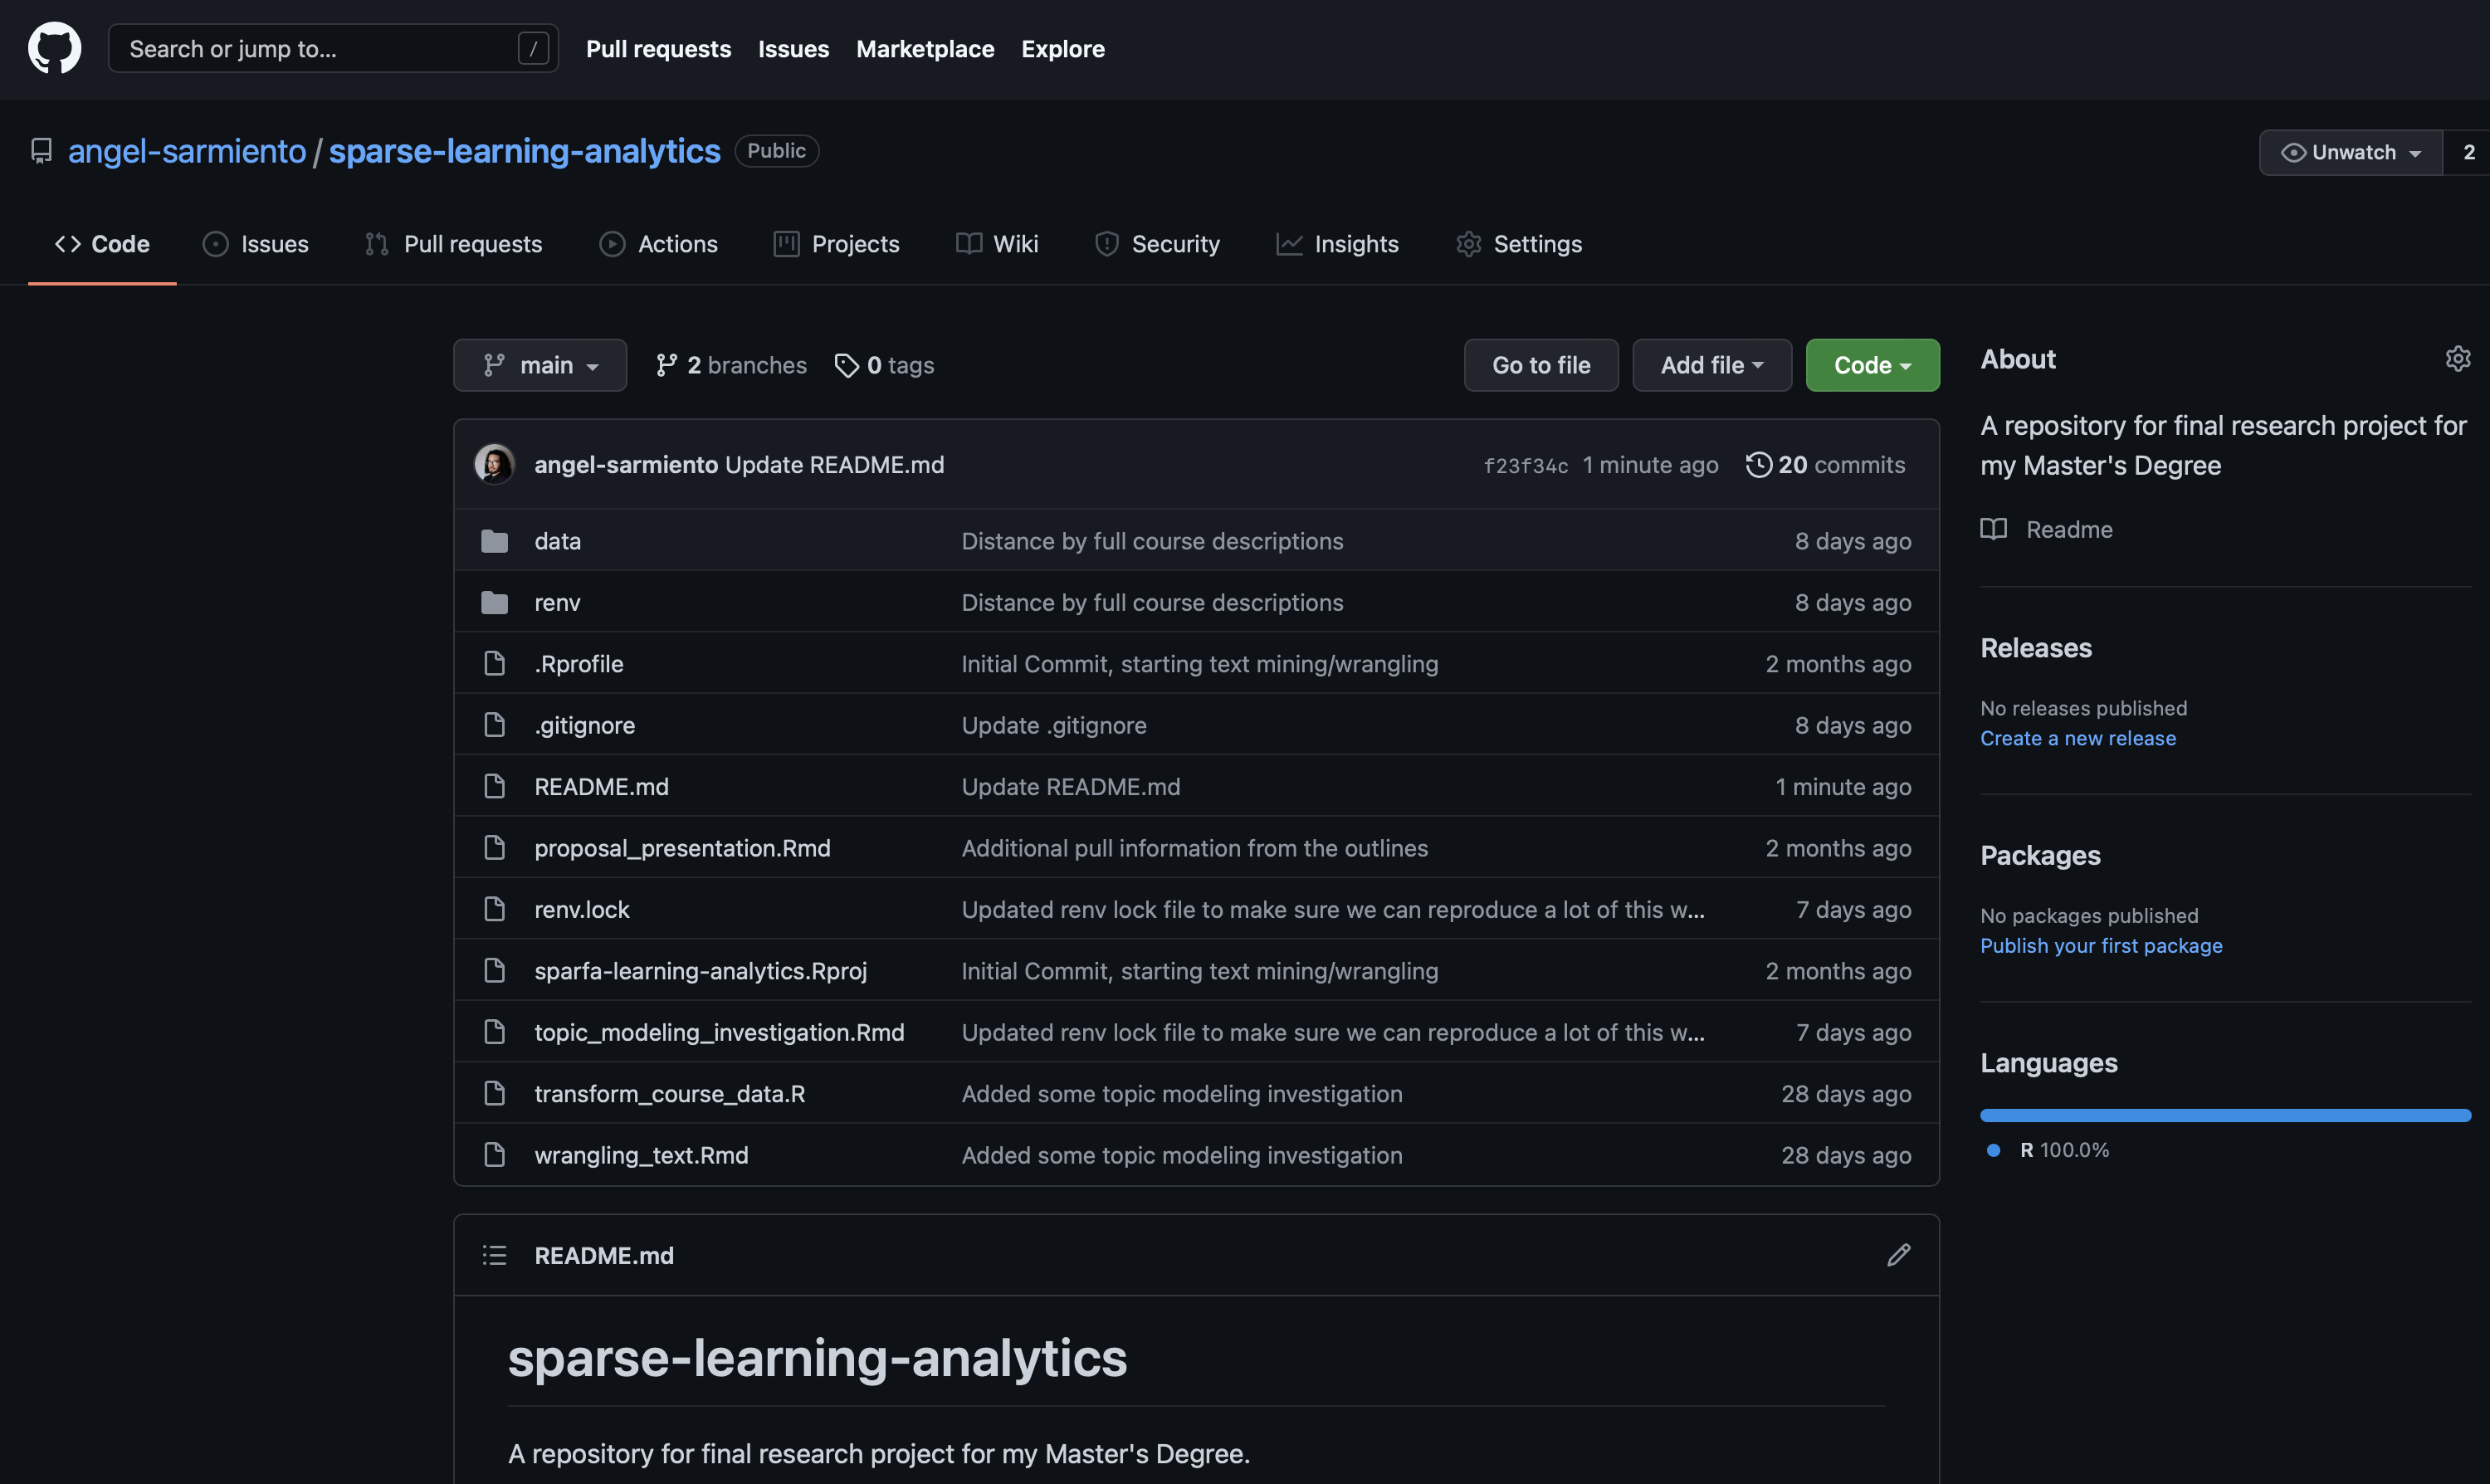
\includegraphics[width = 1\textwidth, height = .6\textheight]{Content/images/repo.png}
\caption{Open-source GitHub repository}
\label{fig:repo}
\end{figure}


\section{Correspondence Analysis}
\label{ca} 

The project started with implementations of MCA on bigrams of the course outlines,  first cleaning the data using regular expressions 
\cite{regex} and custom functions.  The 4 latent dimensions produced from MCA were plotted to show some of the associations created.  Figure \ref{fig:mca_2} 
shows a biplot with the third and fourth latent dimensions


\begin{figure}[H]
\centering

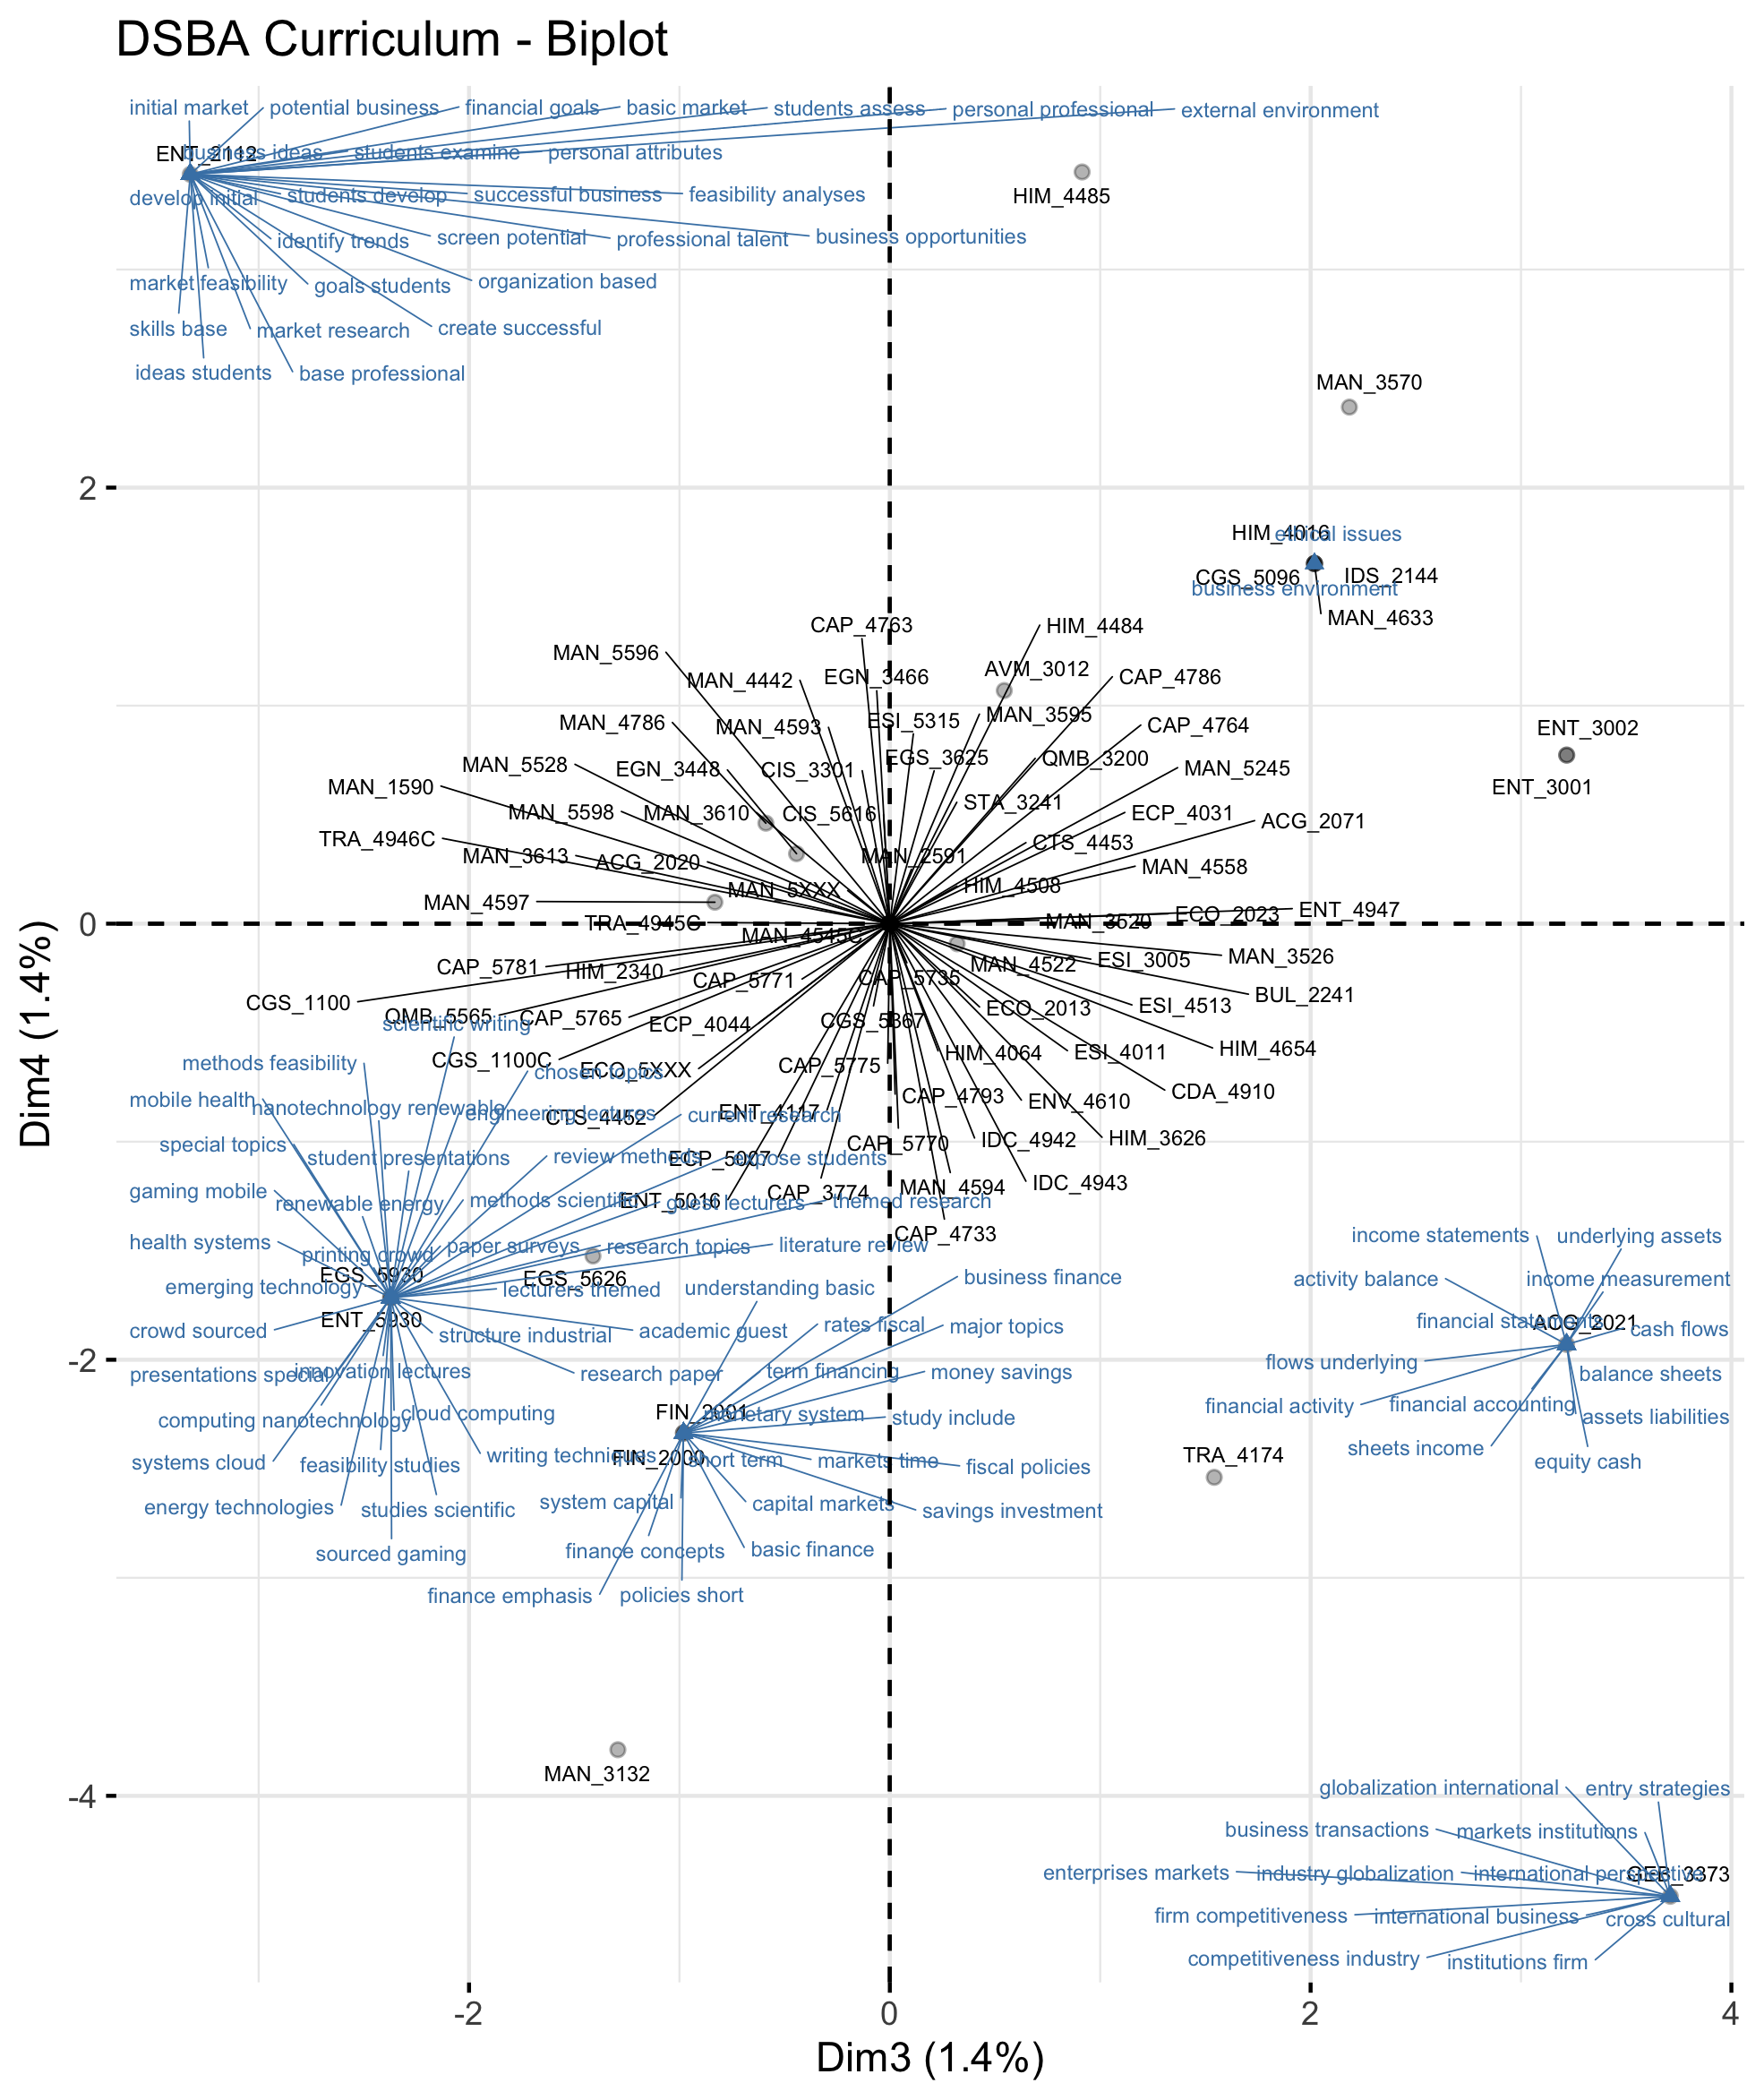
\includegraphics[width = 1\textwidth, height = .9\textheight]{Content/images/mca_bp_2.png}
\caption{Biplot of the DSBA curriculum at FPU,  the top 100 topics and top 30 courses in terms of contribution to the proportion of variance are plotted.}
\label{fig:mca_2}
\end{figure}

Figure \ref{fig:mca_2} shows the potential groupings formed with this methodology.  In the central cluster of courses, a majority of the "MAN" courses occupy 
the second quadrant while the courses heavier in math and programming like statistical learning (STA 3241),  quantitative methods (QMB 3200), and others show 
up in the first quadrant.  The further from the center, the more "niche" the courses (typically business courses like ENT 2112 or ACG 2021) and course topics are.  
This can potentially be used in the future as a backbone to the alignment of course work to corresponding concentrations in the future or as the validation for the 
distance approach discussed later on. 

The plot above only shows a very small subset of the bigrams created from the course outlines since using all of them would not be legible.  Despite this,  
some course-topic association can be seen. EGS 5930 and ENT 5930 are two of the courses that are grouped on the left of the graph, unified by topics like "Cloud Computing" and 
"nanotechnology". 

\section{Latent Dirichlet Allocation}

In developing this project, we wanted to see if well-defined course concentrations were evident from the results of Unsupervised learning techniques applied 
to the text data from the catalog using just the bigrams of the course descriptions.  To do this,  we started with similar data cleaning steps as before, except 
with the course descriptions used to fit a LDA \cite{lda_pap} topic model to identify the 5 different course concentrations in the DSBA curriculum. 

The five concentrations are as follows:   
\begin{itemize}
	\item{Logistics \& Supply Chain Management }
	\item{Intelligent Mobility}
	\item{Quantitative Economics and Econometrics}
	\item{Big Data Analytics}
	\item{Health Systems Engineering}

\end{itemize}

Our topic model was generated with Gibbs sampling for 500 iterations,  getting the document-term probabilities ($\beta$) and ordering in descending order by 
each topic. Figure \ref{fig:lda} shows the results.


\begin{figure}[H]
\centering

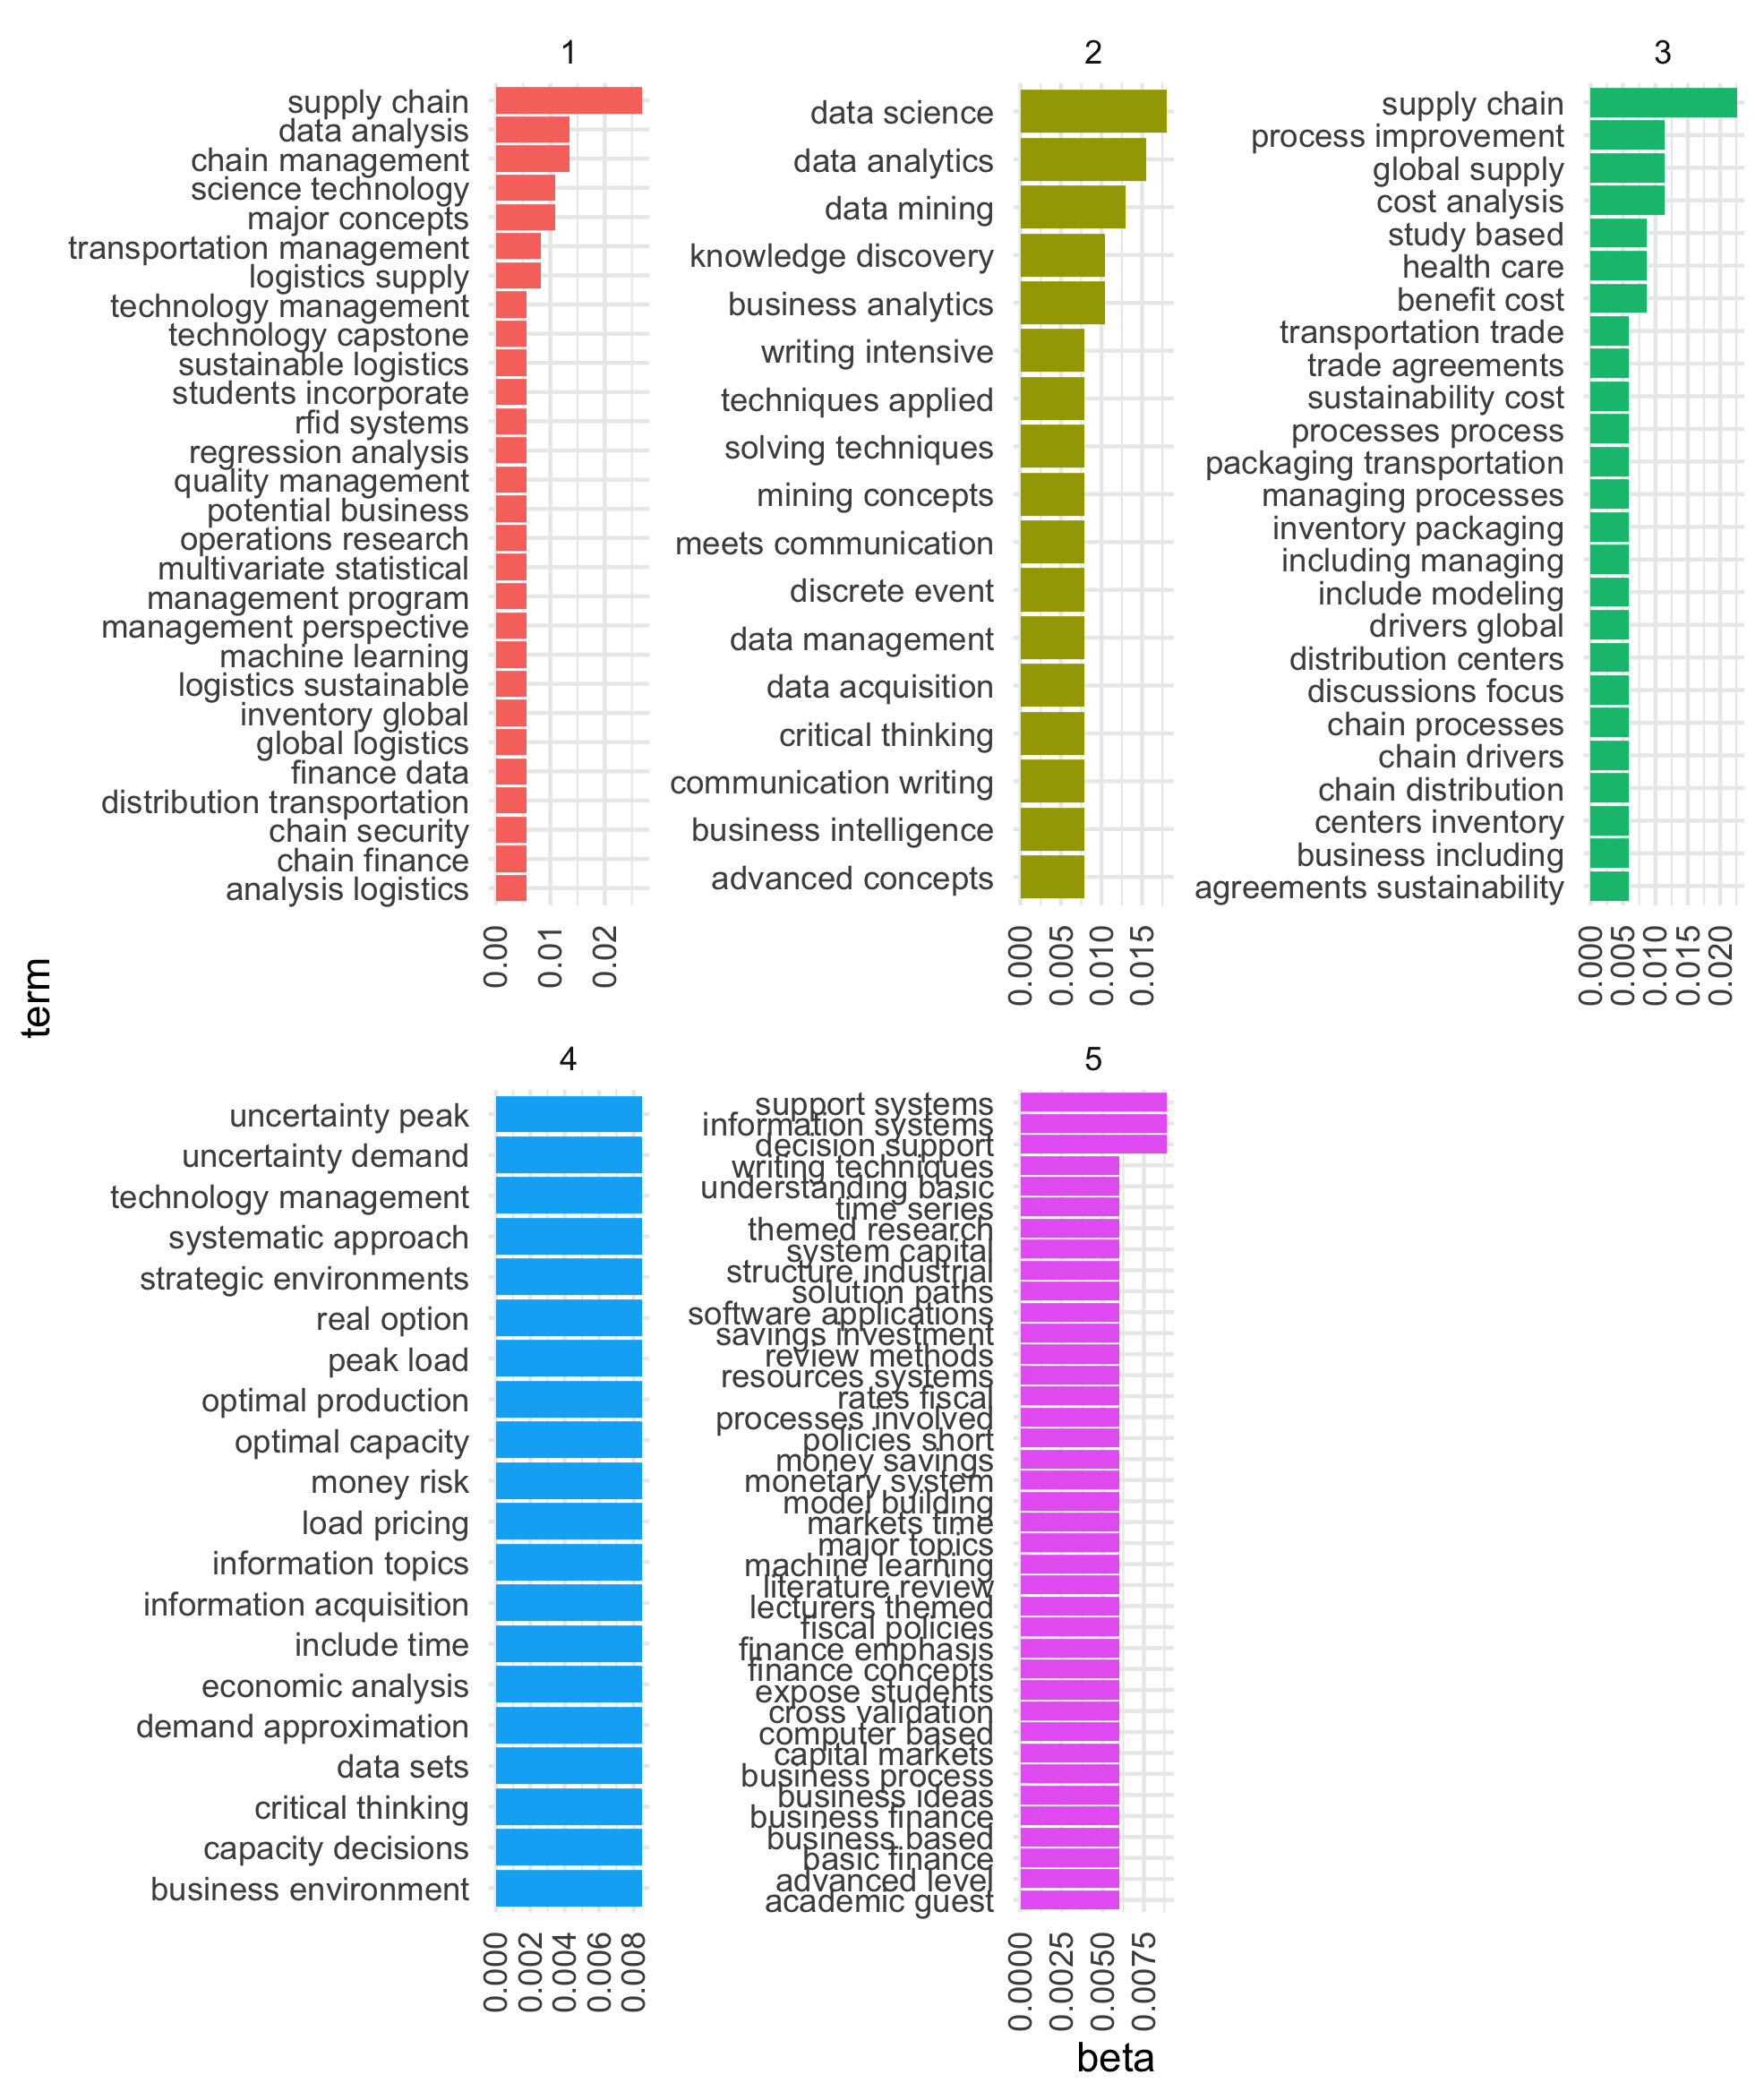
\includegraphics[width = .9\textwidth, height = .8\textheight]{Content/images/lda.png}
\caption{LDA topic model splitting course topics into concentrations}
\label{fig:lda}
\end{figure}

From Figure \ref{fig:lda} above, it is feasible to see that topics 1 and 3 could be in Logistics and Supply Chain Management, topic 4 is most likely Quantitative 
Economics and Econometrics while Big Data Analytics could be topic 2. The segmentation across concentrations is not perfect however, where topics like "machine 
learning" and "regression analysis" show large betas in topic 1, while not being shown in other topics like topics 2 and 4 where one might think to find them 
very proliferate. This seems to be a limitation on the course descriptions and how they differ in size from course to course.  

The beta values represent the \textit{topic-word density}, meaning that higher betas represent a higher number of words that make up a topic.  A lower beta value 
places more weight on fewer, more "dominant" words in the corpus.  Conversely,  higher betas for topics indicate that the topic is assumed to made of up \textit{most} 
of the words in the entire corpus.  For topics 1 and 2 in Figure \ref{fig:lda}, we see that "supply chain" has the highest beta value. This implies that this bigram 
appears very often in the overall corpus of bigrams in the entire dataset and that supply chain is highly likely to be in one or both of those topics.  Topic 5 is 
filled with bigrams with very small beta values in comparison,  implying that something like "capital markets" does not appear very often in the overall corpus 
with a beta value of around $0.0055$,  but groups with other less prevalent words in defining this topic.  Since topic 5 relies on a set of bigrams that do not 
appear as much in the overall dataset, it possibly implies that these bigrams or concepts are niche relative to the entire catalog of concepts.


\section{Multidimensional Scaling}

In order to develop association graphs, we created multiple distance matrices using a variety of different distance metrics.  Some of the distance metrics we used are: 
\begin{itemize}
\item Euclidean distance  
$$\sqrt{\Sigma_{i = 1}^{k}(x_i - y_i)^2}$$
where $x_i$ and $y_i$ are two corresponding documents (course descriptions or outlines) split into vectors of bigrams or vectors containing the full descriptions.
\item Cosine similarity
$$ \cos (\theta) = \frac{A \cdot B}{|| A || || B||}$$
where $\theta$ is the angle between two objects, denoting the similarity.  $||A||$ and $||B||$ are the Euclidean Norm or length of two vectors (in this case, 
course descriptions or course outline vectors). $A \cdot B$ is the dot product  between two course descriptions or course outlines. 
\item Jaccard similarity  
$$\frac{A \cap B}{A \cup B}$$
where A and B are course descriptions or course outlines in vector form, and we are calculating the intersection divided by the union between the two vectors.
\item Burrow's Delta  \cite{burrow}
$$\Delta_B = \Sigma_{i = 1}^n | z_i(D_1) - z_i(D_2)|$$
where $z_i(D) = (f_i(D) - \mu_i/\sigma_i)$ or the standardized z-score for document $D$ and word $i$.  Word frequencies then follow the distribution described 
by Zipf's law \cite{zipf2013psycho}. 

\end{itemize} 

We experimented in plotting relative distances of courses based on the pairwise distance between all of the courses' full course descriptions (not bigrams).  
We used whole course descriptions to combat the potential weaknesses in the n-gram approach not including the entire context of the descriptions.   
Figure \ref{fig:tile} shows a comparison between Jaccard and Cosine distances, the two metrics that resulted in better performance in terms of interpretability,  
for the text data considered in this study. Both of these metrics show mostly defined groupings and display interesting insights. The lighter color of the 
line connecting two courses, the further the distance between them.


\begin{figure}[H]
\centering
\begin{subfigure}{.5\textwidth}
  \centering
  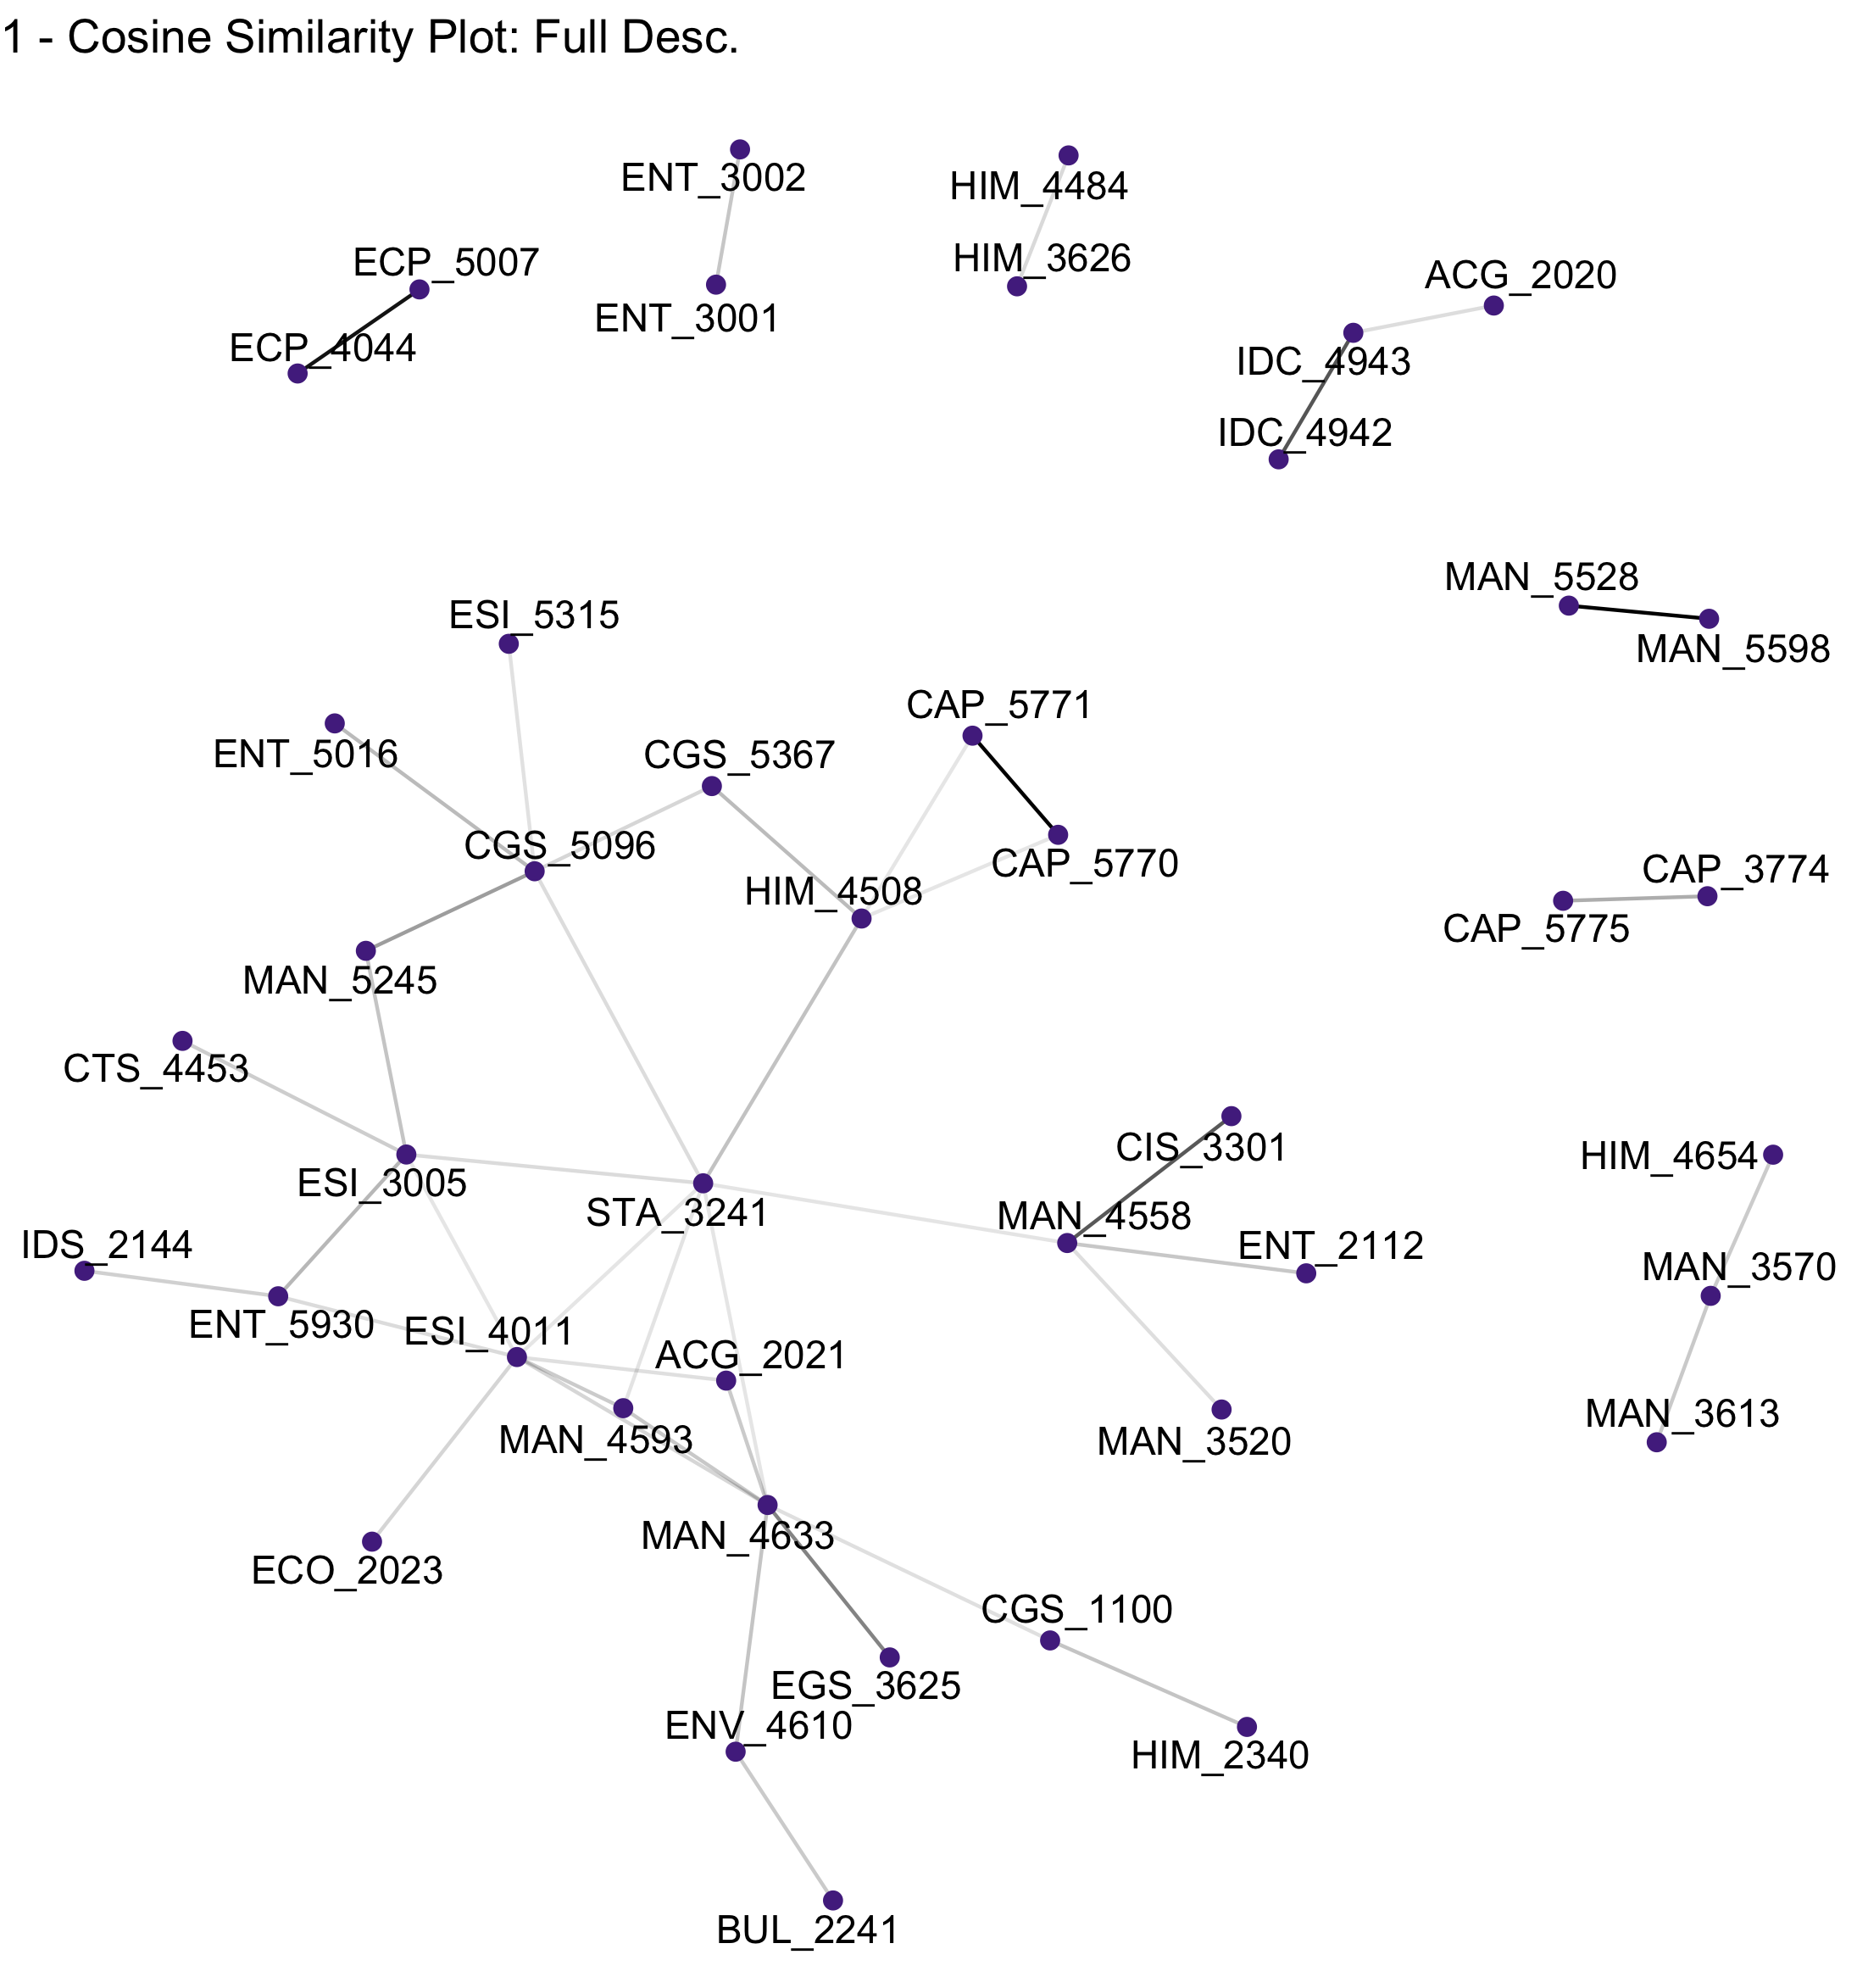
\includegraphics[width=1\linewidth]{Content/images/cos.png}
  \caption{Cosine Distance}
  \label{fig:cos}
\end{subfigure}%
\begin{subfigure}{.5\textwidth}
  \centering
  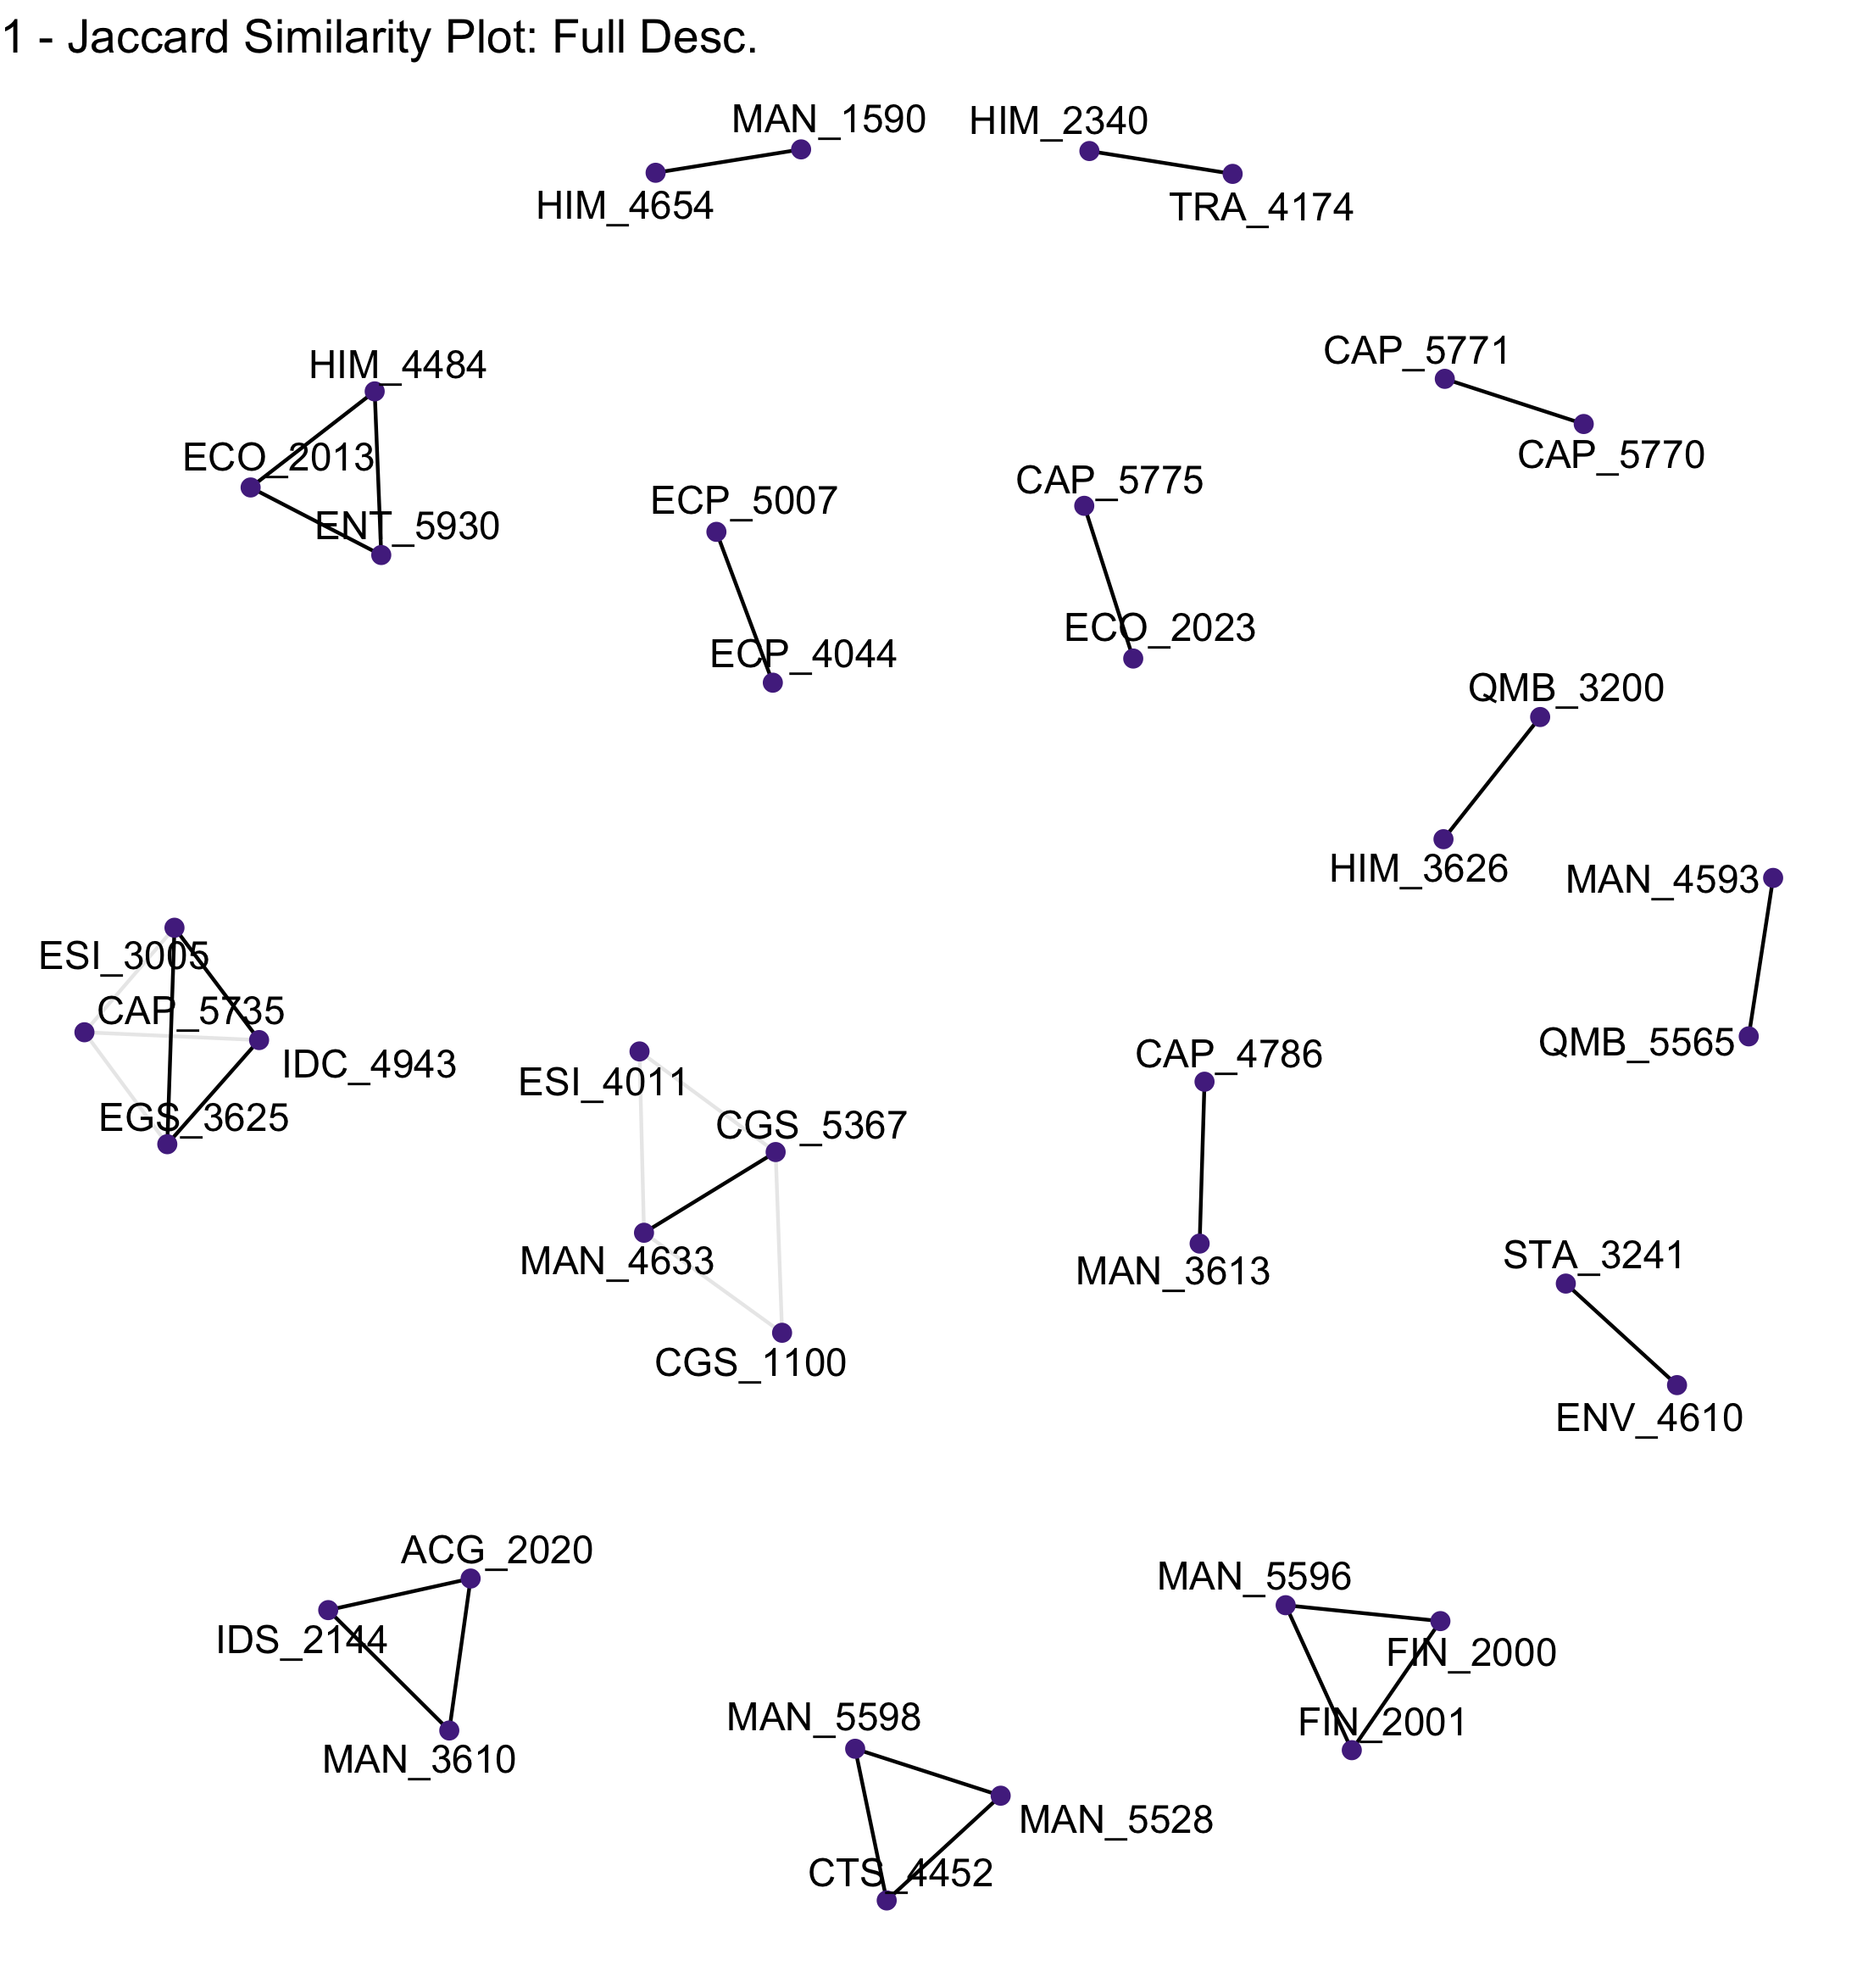
\includegraphics[width=1\linewidth]{Content/images/jac.png}
  \caption{Jaccard Distance}
  \label{fig:jac}
\end{subfigure}
\caption{Comparison between the two best distance metrics}
\label{fig:tile}
\end{figure}

One common trait that became prevalent was the existence of common strings at the end of certain courses.  A majority of the courses that meet a writing 
requirement have the same course descriptions detailing:

 \textit{"This course meets communication/writing-intensive requirements (W)"} 
 
This seems to cause certain courses to be grouped together (have a smaller distance between them).  This is relatively consistent across the catalog and can 
be seen at the bottom of the plot on Figure \ref{fig:cos} with courses like ECO 2013. 

These distance matrices can then be used to apply a method like MDS to separate courses into clusters in latent spaces similar to section \ref{ca}. Ideally, 
we should see relatively defined groupings where we can make inferences on the placement of the courses within those groupings within the latent dimensions.  
Figure \ref{fig:tile2} shows the same distance metrics in Figure \ref{fig:tile} used in our MDS implementation.

\begin{figure}[H]
\centering
\begin{subfigure}{.5\textwidth}
  \centering
  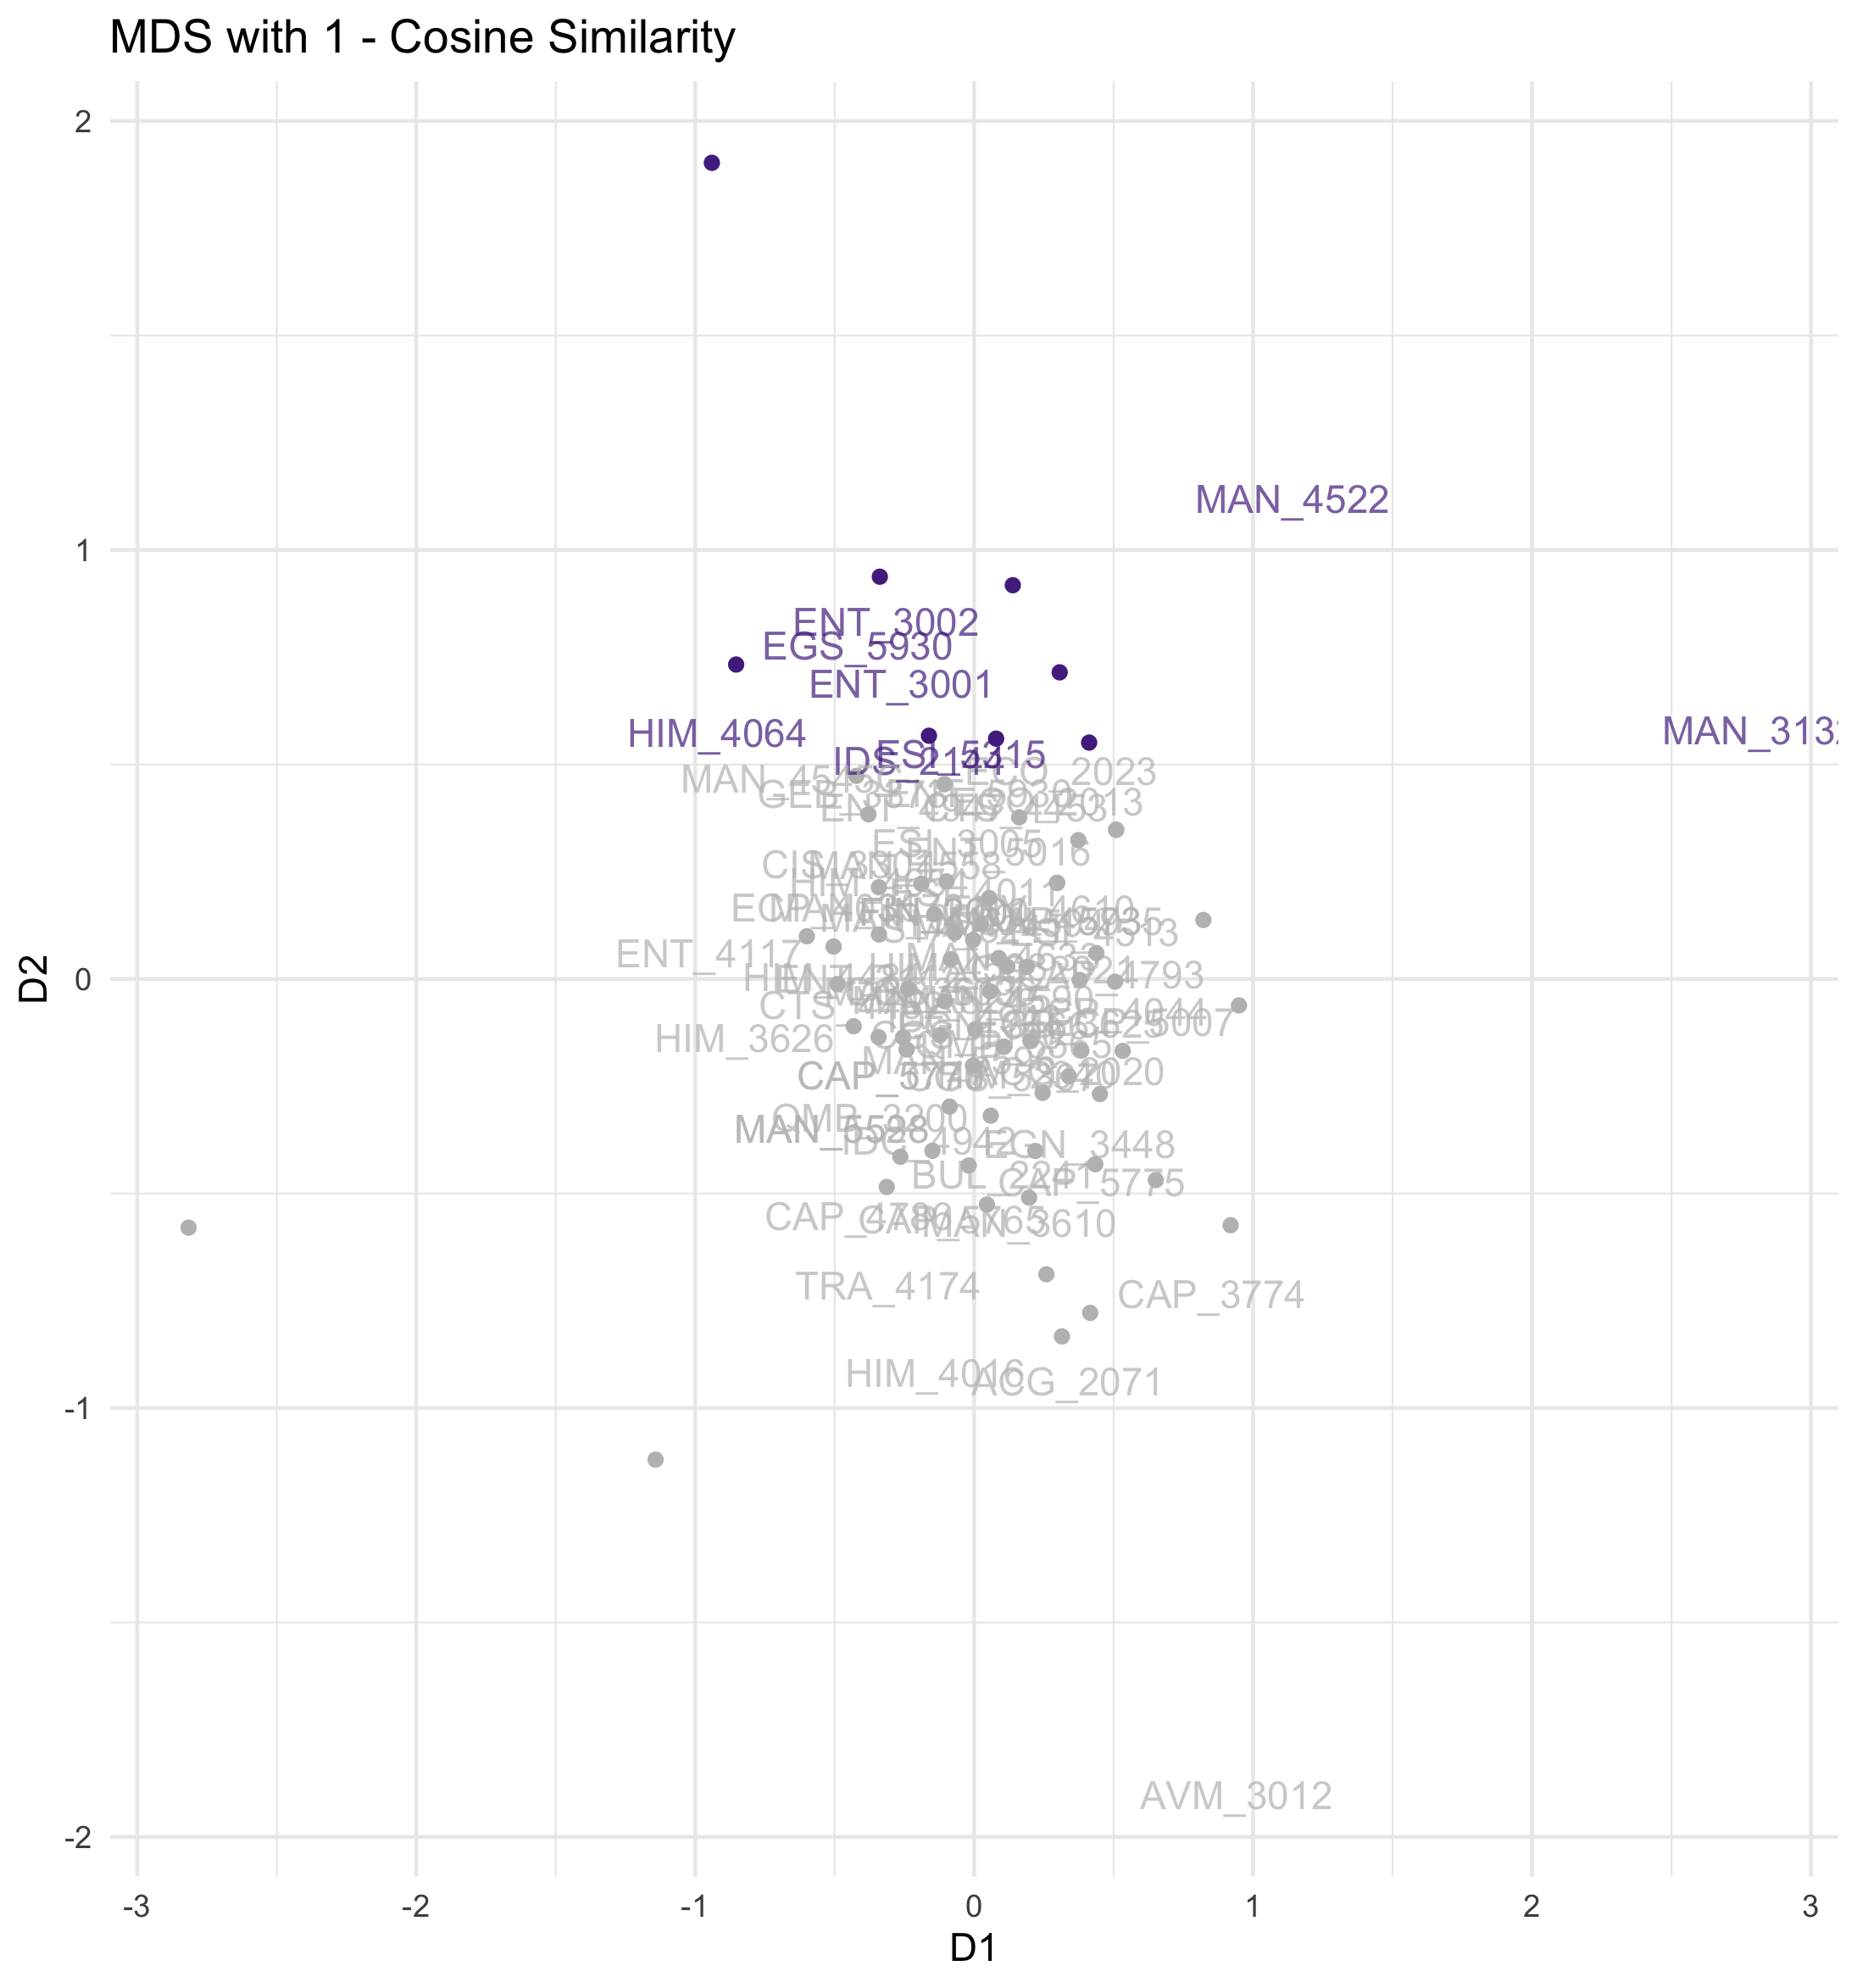
\includegraphics[width=1\linewidth]{Content/images/cos_mds.png}
  \caption{Cosine Distance}
  \label{fig:cmds}
\end{subfigure}%
\begin{subfigure}{.5\textwidth}
  \centering
  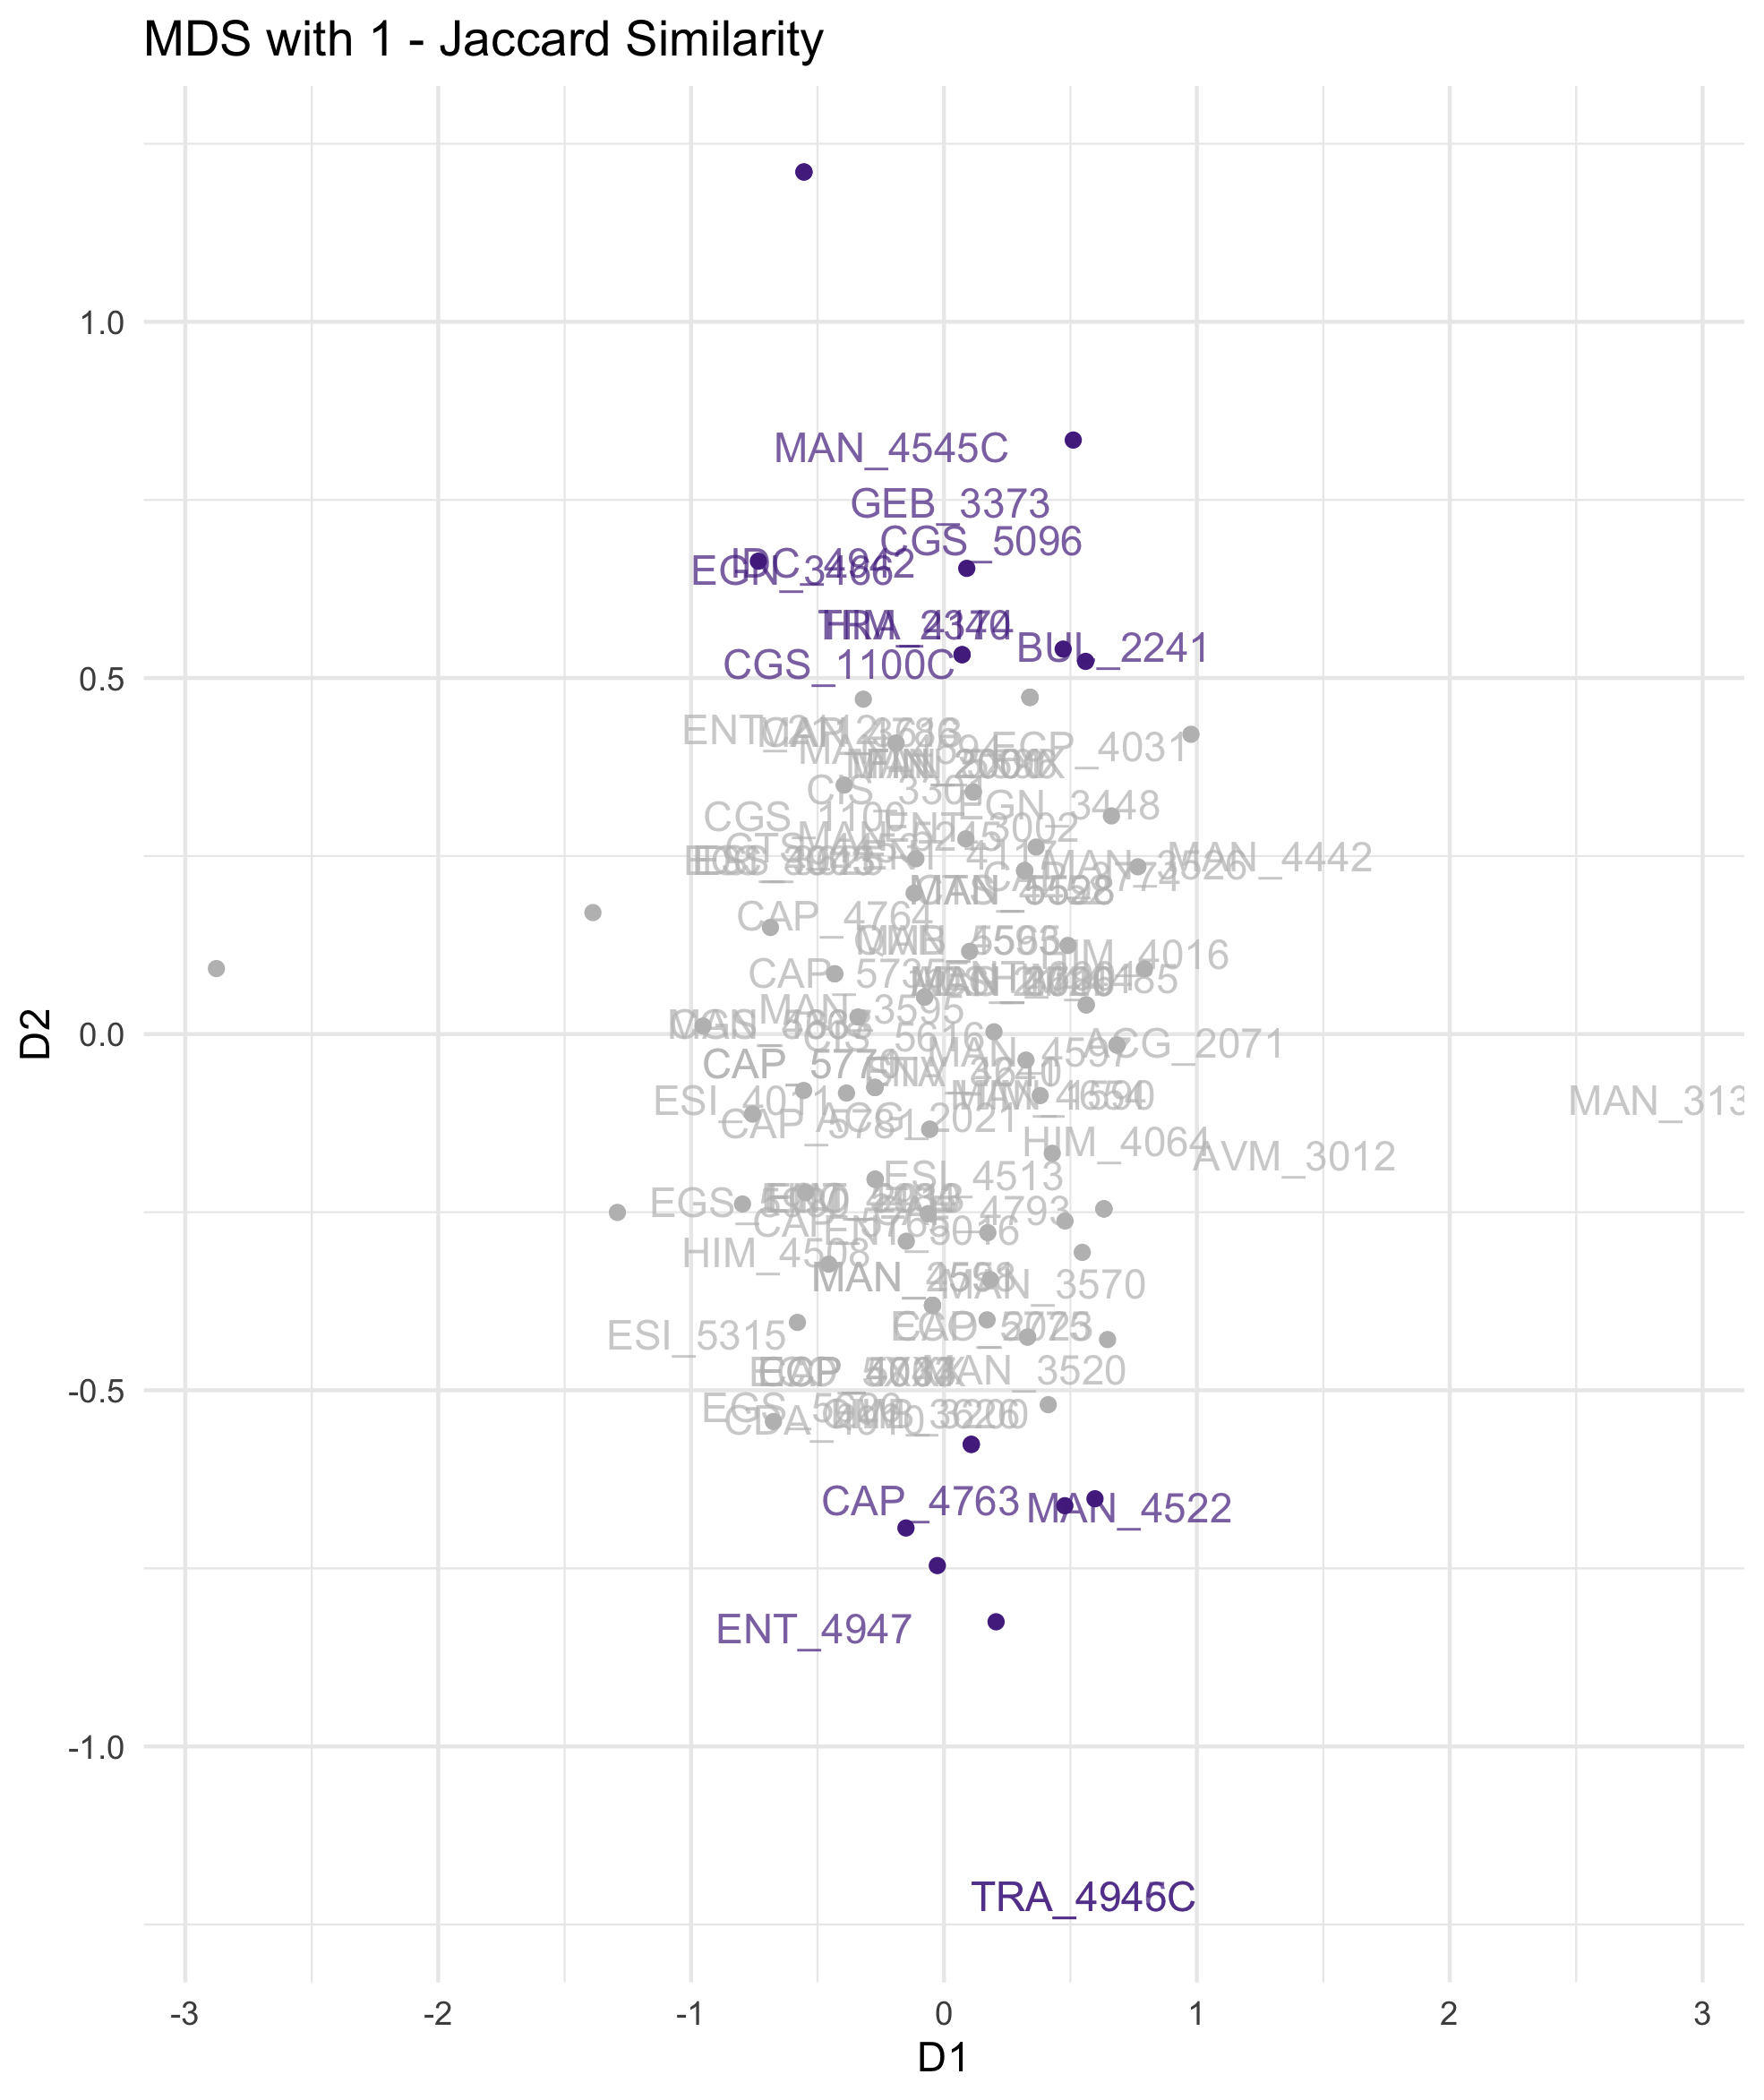
\includegraphics[width=1\linewidth]{Content/images/jac_mds.png}
  \caption{Jaccard Distance}
  \label{fig:jmds}
\end{subfigure}
\caption{Comparison between MDS with Cosine distance and Jaccard distance}
\label{fig:tile2}
\end{figure}

From these plots we see that a grouping separation does not occur.  A majority of the courses group together in the middle within forming those defined 
groupings that one might want to see. A potential reason for this may be the choice of distance metrics. in the future, other distance metrics might prove 
better for providing the segmentation necessary to differentiate the courses using this full course description approach.  Another potential reason could be 
the size of q-grams used to compute the distances for each of the course descriptions: it is possible that different sized substrings might yield better results 
when computing the distance matrices. Increasing the size of the q-grams could potentially give the MDS dimensions more "context" from the larger substrings 
used to compute distances for MDS. 


%\section{Project Schedule}

%\begin{figure}[H]
%\centering

%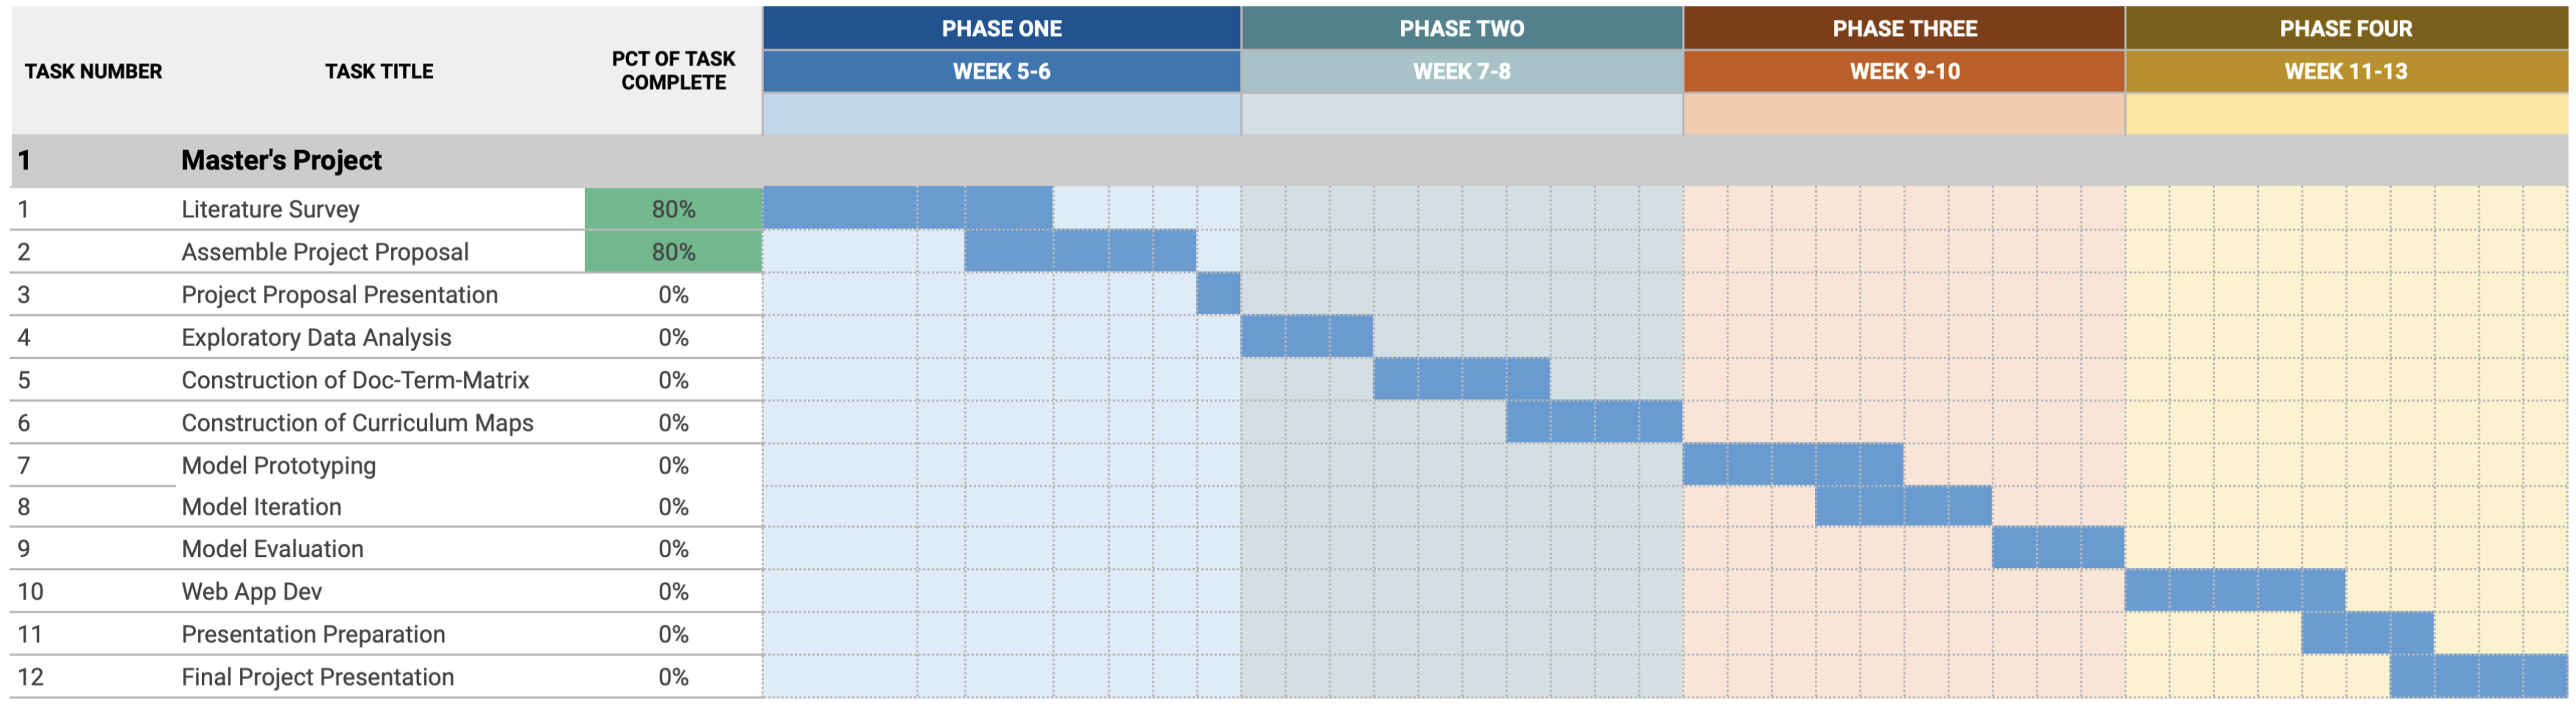
\includegraphics[width = \textwidth]{../images/schedule.png}
%\caption{Project Roadmap/ Gannt Chart}
%\label{fig:diagram}
%\end{figure}

\section{CS Plans of Study}

We can see how these models apply to the Computer Science plan of study as well. Figure \ref{fig:lda_cs} shows the LDA topic 
model and its ability to segment topics detected in the course outline bigrams into the 6 different concentrations present in CS (versus 5 concentrations in 
DSBA as we saw before). 
The concentrations for the CS plan of study are: 

\begin{itemize}
  \item Advanced Topics  
  \item Game Development \& Simulation  
  \item Information Assurance \& Cyber Security  
  \item Software Engineering   
  \item Autonomous Systems  
  \item Big Data Analytics  
\end{itemize}

\begin{figure}[H]
  \centering
  
  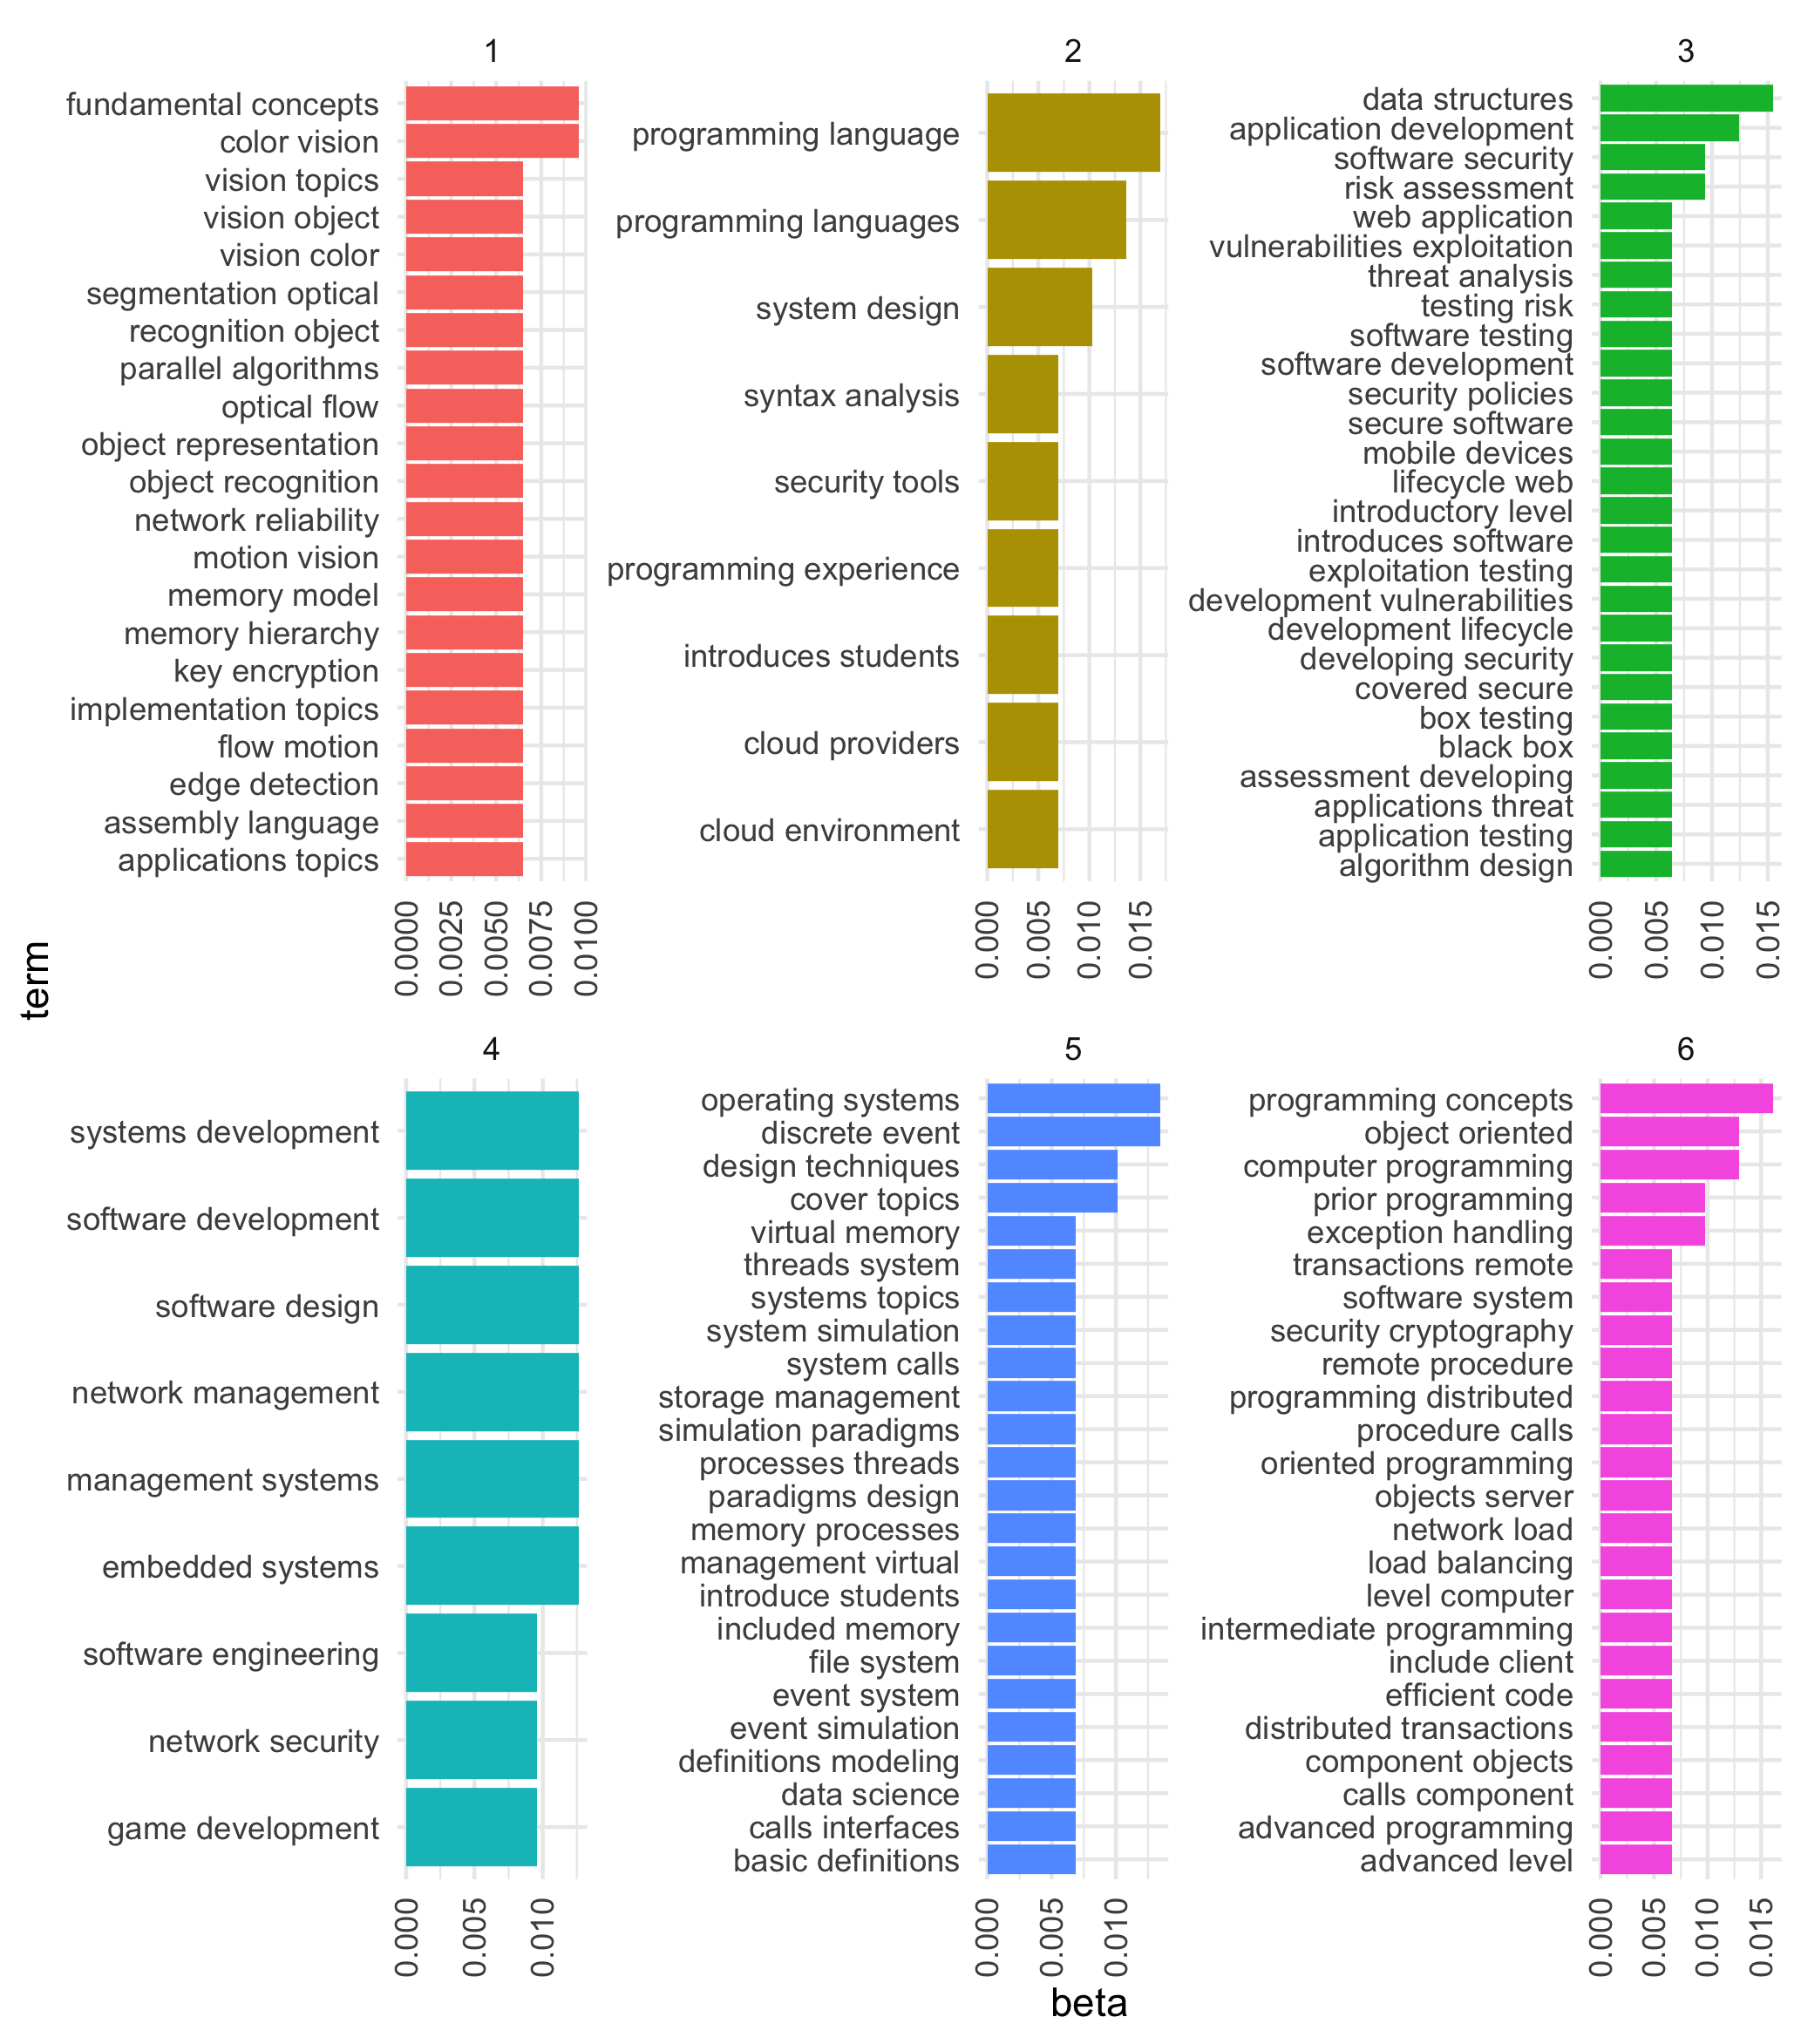
\includegraphics[width = .8\textwidth, height = .7\textheight]{Content/images/lda_cs.png}
  \caption{LDA topic model splitting course topics into concentrations for the Computer Science Plan of Study}
  \label{fig:lda_cs}
\end{figure}

Topic 6 seems to most likely be either Software Engineering or Advanced Topics with terms like "object oriented" and "remote procedure" while topics 2 and 3 fit with Big Data 
Analytics and Cyber Security respectively. Topic 1 has terms that can be aligned with Autonomous Systems like "objection recognition", 
memory model", and "edge detection". 

We can also see how using the cosine similarity works in segmenting the courses based on their full descriptions. Figure \ref{fig:cos_cs} 
shows these results. 

\begin{figure}[H]
  \centering
  
  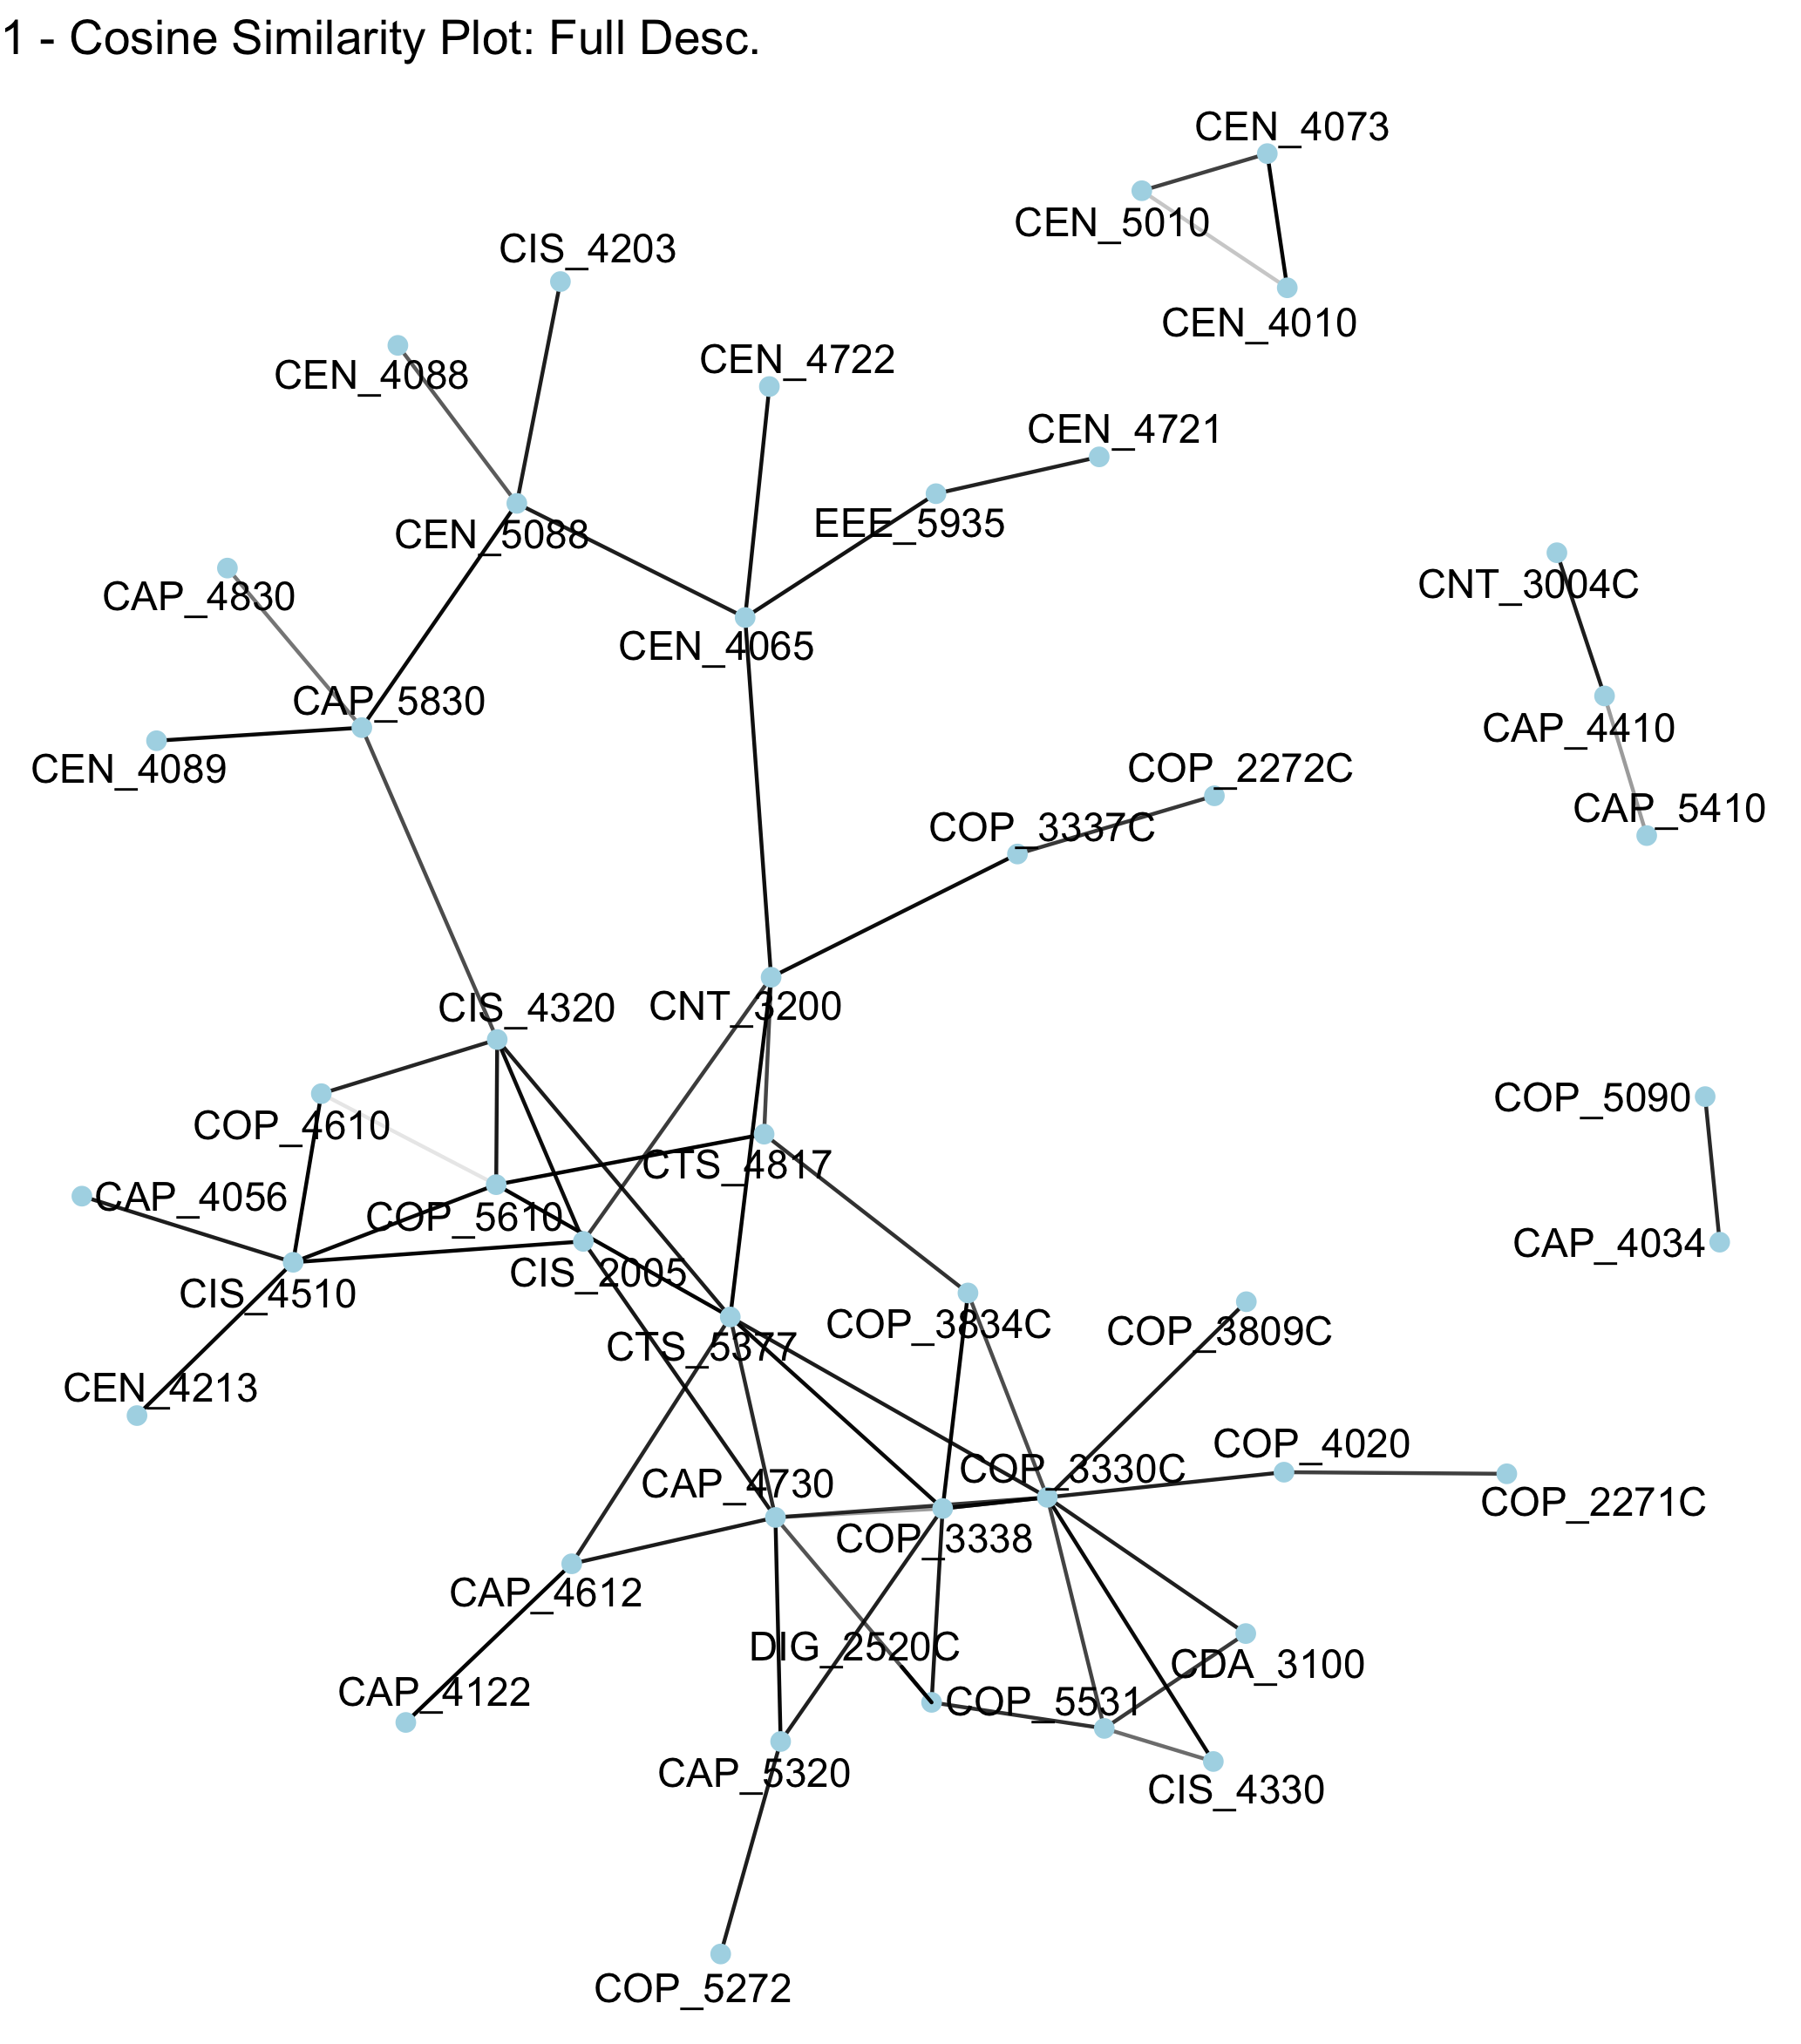
\includegraphics[width = .8\textwidth, height = .7\textheight]{Content/images/cos_cs.png}
  \caption{Cosine distance plot for Computer Science plan of study}
  \label{fig:cos_cs}
\end{figure}

We can see the CEN classes (Software Engineering, Software Design and Architecture, etc.) group together at the top of the plot. 
Where as COP 3330C (Computer Programming 2) Lies at the center of a particularly large grouping at the bottom of the plot. 
This lines up since COP 3330 happens to be either a pre-requisite or co-requisite to the courses it is closest too. The MDS 
biplot can be seen in Figure \ref{fig:cmds_cs}

\begin{figure}[H]
  \centering
  
  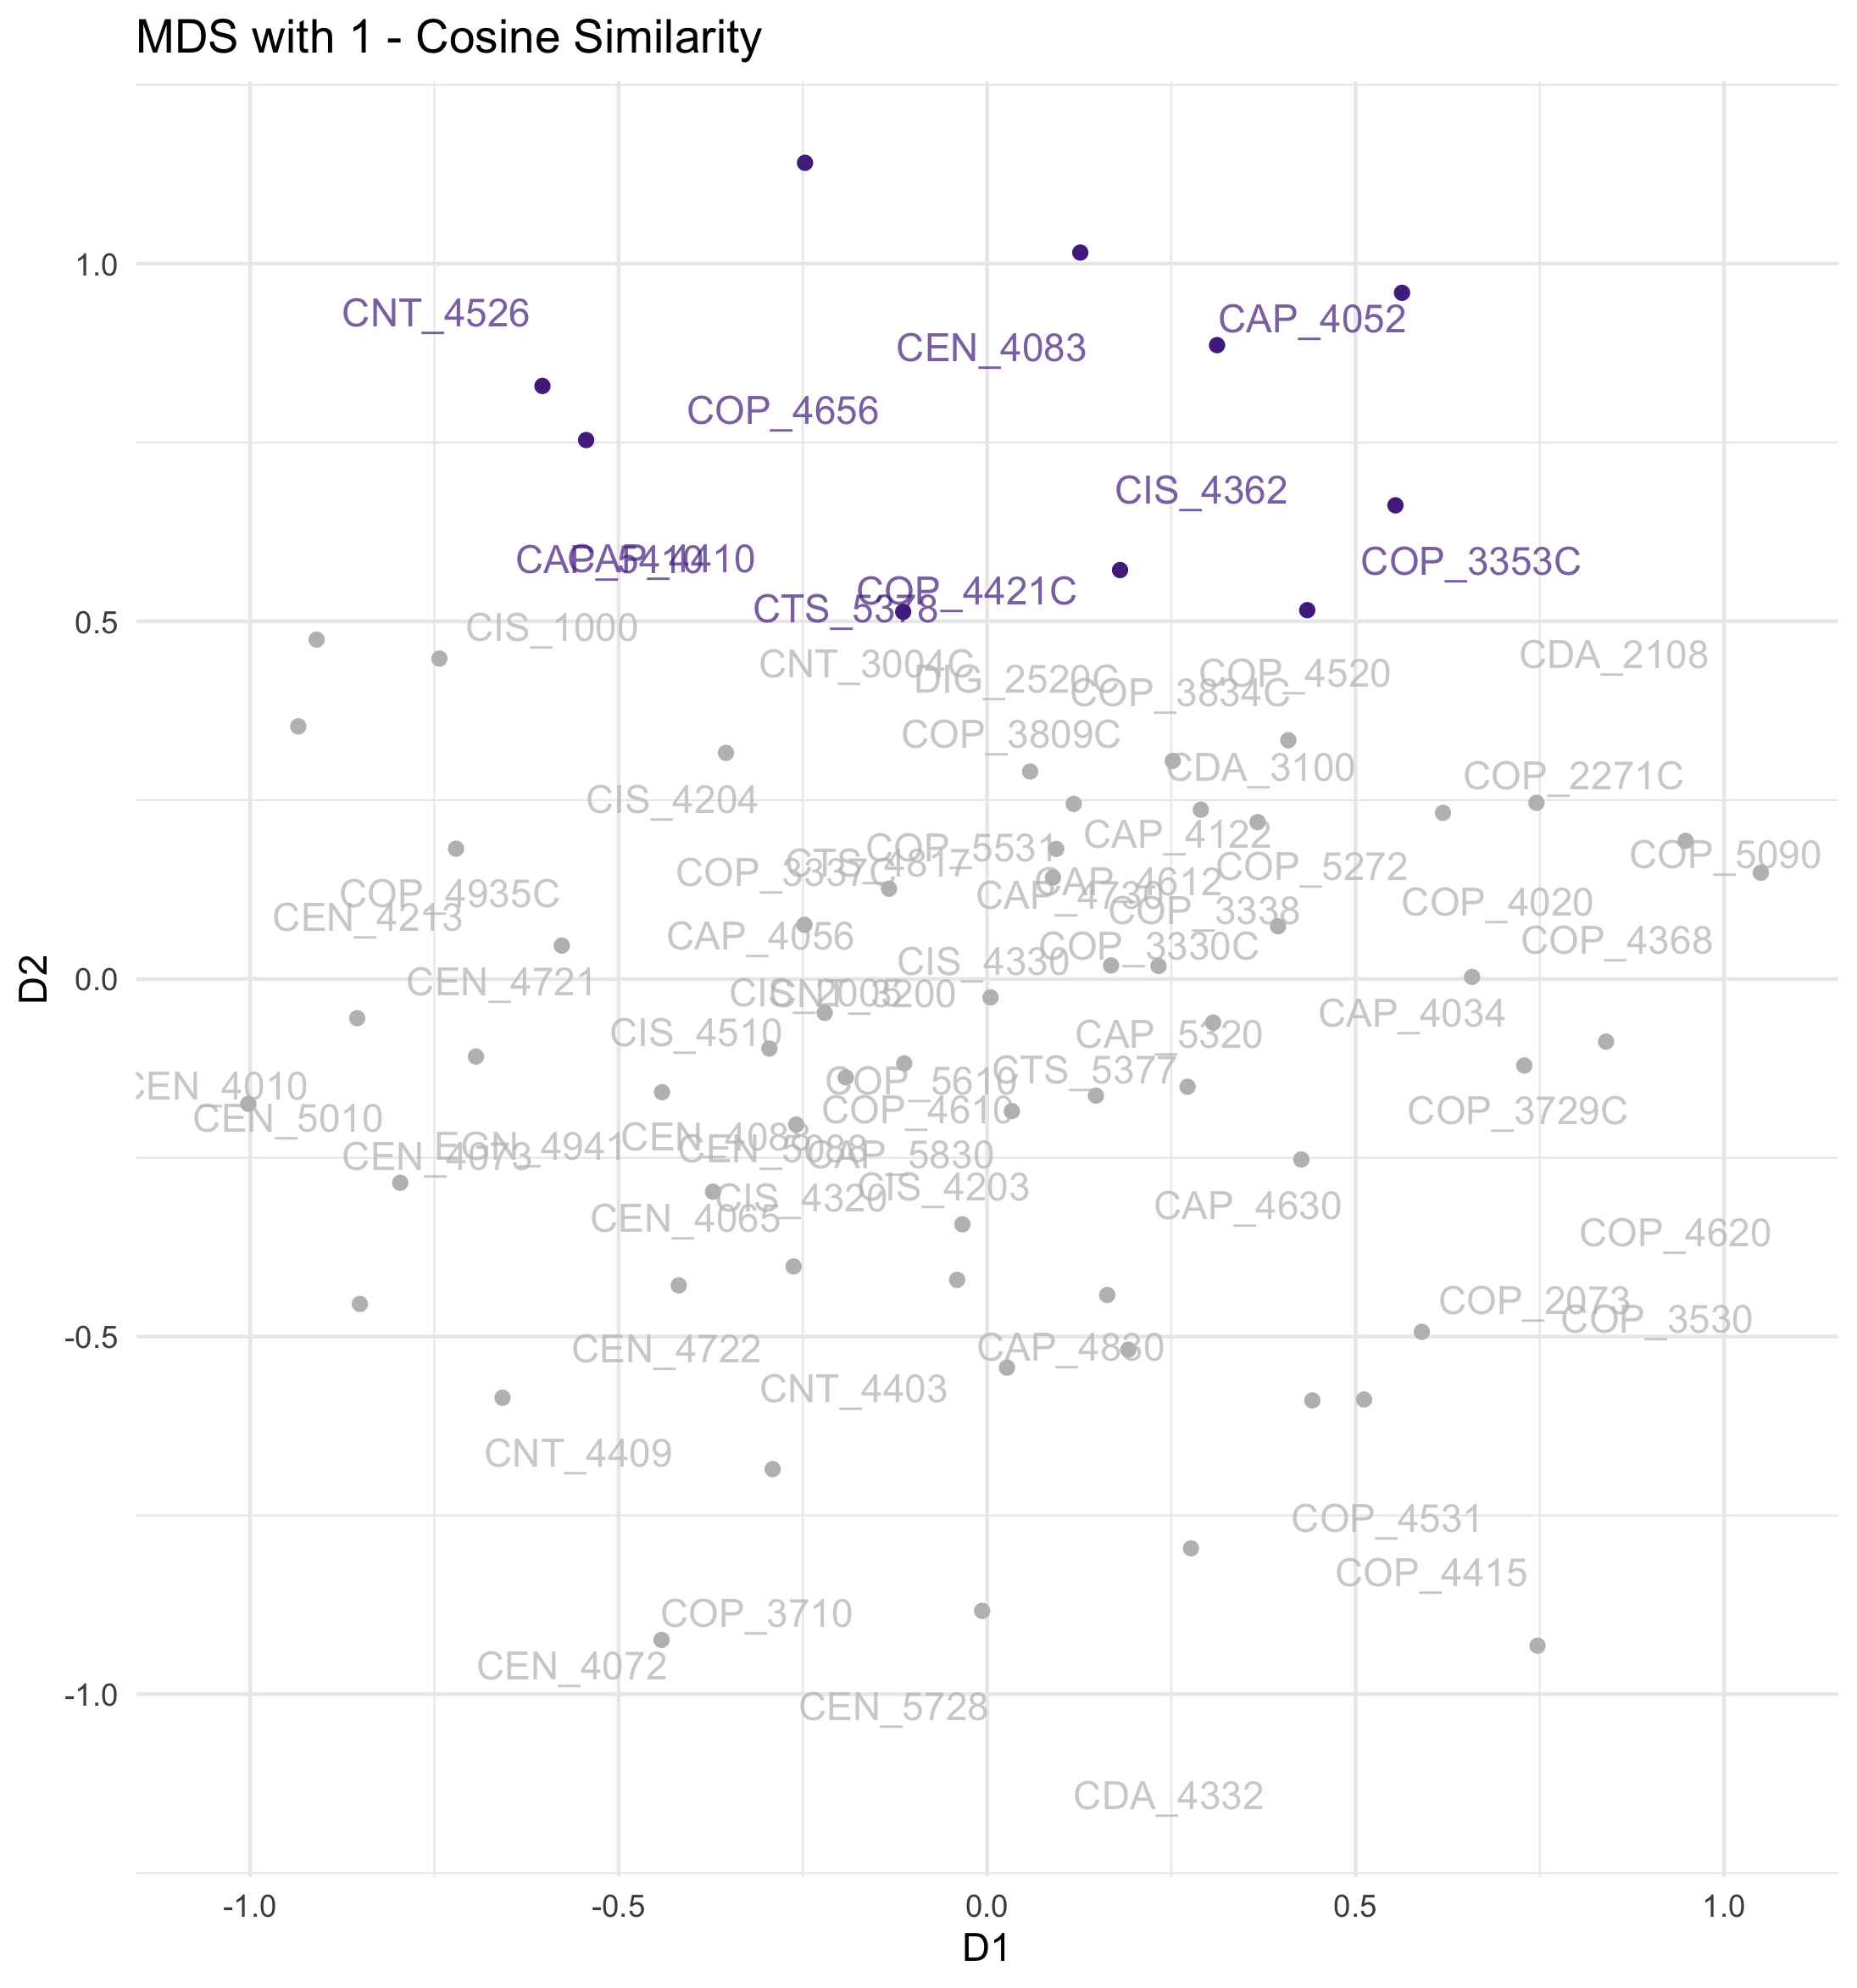
\includegraphics[width = .8\textwidth, height = .7\textheight]{Content/images/cos_mds_cs.png}
  \caption{MDS Results for Computer Science plan of study}
  \label{fig:cmds_cs}
\end{figure}

This results in a much wider distribution across the two latent dimensions from MDS. There seem to be a larger quantity of 
"niche" or non-fundamental classes within CS as a whole, where courses like Advanced Computer Vision (CAP 4410) and 
System Architecture (CDA 4332) can exist toward the outer edges of the catalog. Both of these courses are electives that can be taken 
as concentration courses. 
